\chapter{Méthodologie simple pour l'analyse de performance et le portage de code}
\label{chap:methodo}
\minitoc

Le chapitre précédent présente les différents outils développés durant le travail de thèse. Ces outils ont pour objectif d'aider le programmeur dans sa démarche de caractérisation d'architecture et d'optimisation d'applications. Dans ce chapitre nous proposons une méthodologie à suivre pour réaliser ce travail. La \autoref{sec:methodo_intro} présente les motivations qui nous ont poussé à développer une telle méthodologie. Les cinq sections suivante correspondent aux cinq étapes de la méthodologie



\section{Introduction}\label{sec:methodo_intro}

À cause des pressions énergétique et économique, les plateformes de calculs haute performance doivent être repensées. De nouvelles architectures optimisées pour certaines applications devront être utilisées rendues possibles grâce au protocole Gen-Z. En l'absence de méthode de caractérisation fine de la performance des codes, ces architectures inovantes sont potentiellement condamnées puisque peu d'experts savent les valoriser. Cependant, ces nouvelles architectures très différentes de celles utilises aujourd'hui (x86, GPU) doivent être caractérisées pour prédire le gain de performance pour les applications. Pour pouvoir profiter de ces technologies et les utiliser de façon optimale, nous avons présenté dans le chapitre précédent une suite de logiciels de caractérisation et d'analyse de performance. L'objectif de ce chapitre est de présenter une méthodologie adaptée,  permettent de réaliser cette caractérisation ainsi que le portage des applications sur ces nouveaux accélérateurs.



\subsection{La révolution de l'hétérogénéité}
%%%%%%%%%%%%%%%%%%%%%%%%%%%%%%%%%%%%%%%%%%%%%%%

    Le protocole Gen-Z, présenté dans le chapitre \ref{sec:edl_hpc}, va révolutionner le monde de l'informatique comme peu de technologies auparavant. Entre tous les bénéfices apportés par ce protocole, la faculté de rendre facile l'hétérogénéité dans les super-calculateurs est sans doute la plus importante. 
    
    L'hétérogénéité sera à la fois entre des accélérateurs spécialisés pour différentes workload, mais aussi dans les architectures elles mêmes permettant de mixer et d'adapter chaque coprocesseur. En 2018, plus de 96\% des processeurs des super-calculateurs du Top500 ont une architecture x86 et la majorité d'entre eux (91\%) proviennent du constructeur Intel. Seulement 28\% des 500 clusters sont associés à des accélérateurs dont 92\% sont des GPU NVIDIA. Nous remarquons donc que l'architecture des super-calculateurs est très similaire et que l'utilisation d'accélérateurs adaptés n'est encore qu'à ses débuts. Aujourd'hui l'utilisation d'architectures différentes est souvent perçu négativement car elle implique d'adapter les codes, d'utiliser plusieurs langages ou d'obtenir de mauvaises performance car l'architecture n'est pas adaptée à la totalité de l'application.
    
    Par analogie, nous comparons cette opportunité avec celle des moteurs d'avion à réaction qui ont révolutionné l'économie et le domaine de l'aviation. Si certains constructeurs et utilisateurs continuent d'utiliser la même stratégie d'ajouter des serveurs \textit{standards} comme jusqu'à aujourd'hui, ils seront dépassés par ceux ayant commencé à investir ces nouvelles technologies plusieurs années avant eux. Il est donc cruciale de s'y préparer en ayant la bonne méthodologie et les bons outils pour pouvoir en profiter. L'accès à des plate-forme exascale et à ces nouvelles architectures va aussi ouvrir de nouveaux marchés, inaccessible aujourd'hui à cause de plusieurs contraintes: le prix, la bande passante nécessaire, la sécurité ou encore la consommation électrique. 
    
    Les gains de performance ne viendront pas seulement par l'utilisation d'accélérateurs puissants, mais de leur diversité et de la capacité des programmeurs de bien les utiliser. Pour une même application, plusieurs accélérateurs spécialisés seront souvent nécessaires. On peut en imaginer certains adaptés à la lecture et à la décompression du jeu de données. Un fois réalisé, des accélérateurs spécialisés dans le calcul demandé pourront être utilisés (ASIC, FGPA ou DSP). Enfin pour la visualisation des données, des GPU seront alors nécessaires. L'hétérogénéité est à la fois un challenge majeur des plate-formes Exascale, mais aussi une grande opportunité. 
    
    

\subsection{Développement}
%%%%%%%%%%%%%%%%%%%%%%%%%%%%%%%%%%%%%%%%%%%%%%%

    Comme présente dans la section \ref{X}, l'analyse de performance peut se faire à plusieurs niveaux. En fonction de l'objectif défini, le niveau et les outils utilisés doivent être adaptés. Notre analyse porte sur la performance d'une partie du code intéressante, un hot spot. Les outils développé permettent pour le moment de mettre en avant des problèmes de performances dus au système mémoire ou au processeur. Les problèmes de performances liés au réseaux ou au système d'exploitation ne sont pas la priorité de la méthodologie, bien qu'ils puissent être décelé.
    
    Du fait de la complexité des architectures, le travail de portage et d'optimisation peut être très difficile. Ainsi, notre démarche s'adresse aux programmeurs ayant de solides connaissances des micro-architectures. Pour améliorer la précision de l'analyse et des outils il est préférable d'avoir accès au code source. 
    
    Contrairement à des solutions existante comme VTune \cite{vtune}, nous avons choisi de développer plusieurs outils indépendant répondant chacun à une question précise. Nous espérons qu'en réduisant la complexité de l'outillage, l'adoption des outils auprès des programmeurs sera plus grande. Les outils n'ont pas vocation d'automatiser entièrement les tâches du programmeur. La puissance de ces outils vient de leur utilisation complémentaire. 
    
    Les outils utilisés sont disponibles en Open Source et ne sont pas exhaustifs. Certains outils utilisés ont été développé durant la thèse, d'autres répondant à nos critères n'ont pas eu à être développés de nouveau. Cette méthodologie et les outils l'accompagnant sont présentés pour partager notre philosophie d'analyse de performance, mais le travail doit être poursuivi pour ajouter de nouveaux outils. De plus, le contexte de leur utilisation est de profiter de l'hétérogénéité arrivant dans les centre de données, ils nécessiteront d'être portés sur ces architectures.



    \begin{figure}
        \center
        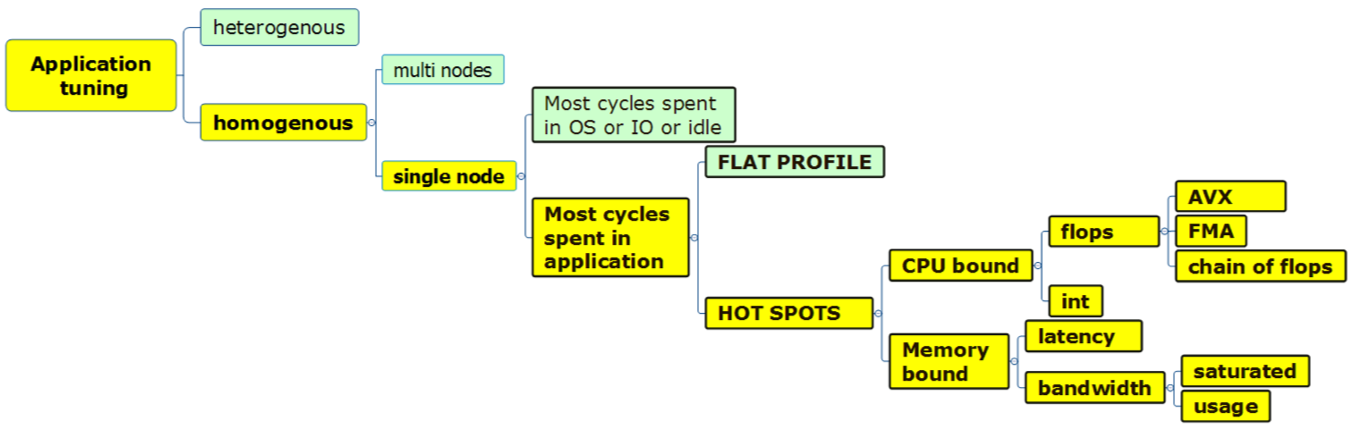
\includegraphics[width=10cm]{images/analyse.png}
        \caption{\label{pic_analyse} Délimitation de l'analyse proposée.}
    \end{figure}

    
    
\subsection{Contributions}
%%%%%%%%%%%%%%%%%%%%%%%%%%%%%%%%%%%%%%%%%%%%%%%

    Dans ce chapitre, nous présentons une méthodologie simple en 5 étapes permettant aux utilisateurs de modéliser les performances de leur code, de les projeter sur de nouvelles architectures et de les optimiser (voir \autoref{pic:methodologie_step_2}). Nous proposons un modèle de performance simple basé sur les caractéristiques du sous-système mémoire. L'objectif est de créer pour chaque \textit{hot spot} un modèle de ses performances dans le but de projeter ses performances sur d'autres architectures mais aussi de valider ses performances. Nous cherchons à prouver la bonne utilisation ou non du système mémoire, ressource critique pour la performance des applications sur les architectures modernes. Enfin, lorsque les performances de l'application ne sont pas celles attendues par notre modèle, nous proposons un cheminement pour comprendre, optimiser et transformer le code pour parvenir aux performances ultimes.

    \begin{figure}
    \center
    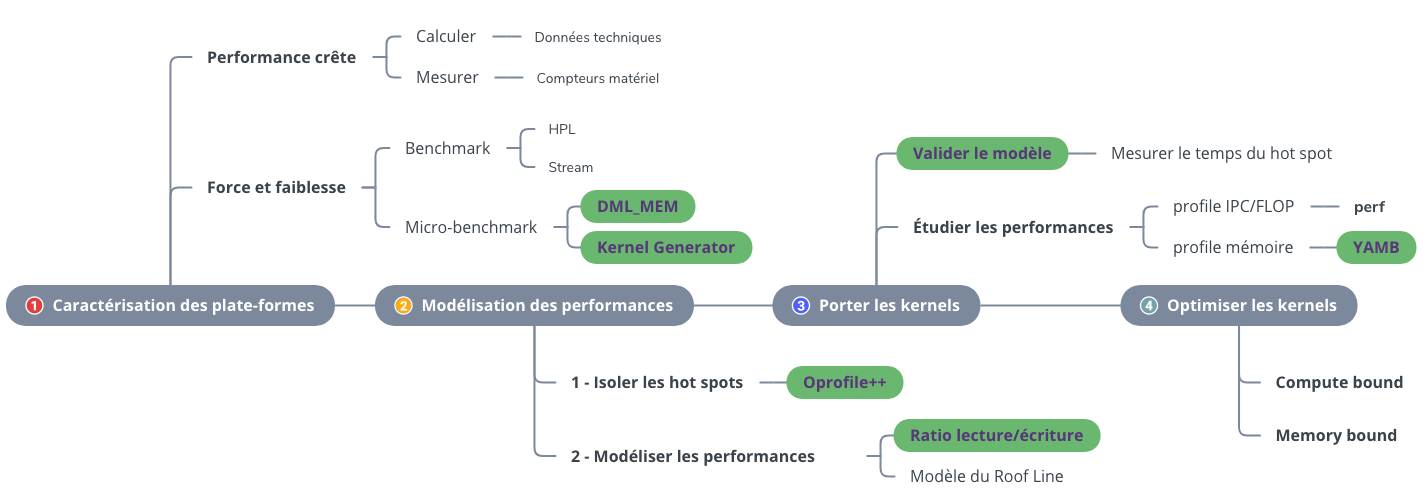
\includegraphics[width=14cm]{images/methodologie_step.png}
    \caption{\label{pic:methodologie_step_2} Méthodologie en 5 étapes pour caractériser et optimiser une application sur une nouvelle architecture.}
    \end{figure}
            
    
    Pour illustrer les différentes étapes, nous appliquons la méthodologie à l'étude des performances de la fonction \textit{triadd} (voir extrait de code \ref{lst:triadd}) du benchmark Stream \cite{McCalpin1995} sur un processeur Intel\textit{ Xeon Gold 6148} possédant 20 coeurs. Les matrices utilisées mesurent chacune 19.6 GB. Cet exercice nous permet de montrer que même pour un code aussi simple et en apparence optimisée, l'approche et les outils utilisés permettent de comprendre et d'optimiser ses performances.
    
\begin{lstlisting}[language=c,caption=Fonction Triadd extraite du benchmark Stream \ref{McCalpin1995},label={lst:triadd}, 
  basicstyle=\footnotesize, frame=tb,
  xleftmargin=.065\textwidth, xrightmargin=.065\textwidth]
for (j=0; j < STREAM_ARRAY_SIZE; j++)
    A[j] = B[j] + scalar * C[j];
\end{lstlisting}


\iffalse 
%%%%%%%%%%%%%%%%%%%%%%%%%%%%%%%%%%%%%%%%%%%%%%%%%%%%%%%%%%%%%%%%%%%%%%%%%%%%%%%%%%%%%%%%
%%%%%%%%%%%%%%%%%%%%%%%%%%%%%%%%%%%%%%%%%%%%%%%%%%%%%%%%%%%%%%%%%%%%%%%%%%%%%%%%%%%%%%%%
%%_______ .___________.    ___      .______    _______                       __       %%
%%|   ____||           |   /   \     |   _  \  |   ____|                    /_ |      %%
%%|  |__   `---|  |----`  /  ^  \    |  |_)  | |  |__          ______        | |      %%
%%|   __|      |  |      /  /_\  \   |   ___/  |   __|        |______|       | |      %%
%%|  |____     |  |     /  _____  \  |  |      |  |____                      | |      %%
%%|_______|    |__|    /__/     \__\ | _|      |_______|                     |_|      %%
%%%%%%%%%%%%%%%%%%%%%%%%%%%%%%%%%%%%%%%%%%%%%%%%%%%%%%%%%%%%%%%%%%%%%%%%%%%%%%%%%%%%%%%%
%%%%%%%%%%%%%%%%%%%%%%%%%%%%%%%%%%%%%%%%%%%%%%%%%%%%%%%%%%%%%%%%%%%%%%%%%%%%%%%%%%%%%%%%
\fi


%%%%%%%%%%%%%%%%%%%%%%%%%%%%%%%%%%%%%%%%%%%%%%%%%%%%%%%%%%%%%%%%%%%
\section{Étape 1: Veille technologique}\label{sec:methodo_step1}
%%%%%%%%%%%%%%%%%%%%%%%%%%%%%%%%%%%%%%%%%%%%%%%%%%%%%%%%%%%%%%%%%%%

%%%%%%%%%%%%%%%%%
\subsection{Motivation et objectifs}
%%%%%%%%%%%%%%%%%

Grâce à Gen-Z, de nouvelles technologies utilisable par les super-calculateurs vont apparaître régulièrement. Comme expliqué précédemment, il est crucial pour les utilisateurs de porter leur code et d'investir du temps et de l'argent dans les bonnes plate-formes. Aujourd'hui ce choix se limité à quelques architectures, principalement les CPU (Intel, AMD, IBM) et les accélérateurs (NVIDIA, AMD, Xeon Phi). Demain, prendre la bonne entre toutes les nouvelles technologies sera beaucoup plus difficile.

Même si elle n'est pas une étape de la méthodologie en soit, le premier travail de développeur est d'être en constante recherche des dernières innovations technologiques. Cela peut être de nouveau processeurs, de nouvelles mémoire ou bien de nouveaux algorithmes ou optimisations. Il est très important de se tenir à l'état de l'art ou même en avance pour anticiper les nouveautés. 

Le but principal de cette étape est de répertorier toutes les plate-formes et technologies potentiellement intéressantes pour le calcul haute performance. Certaines caractéristiques clés sont calculées à partir des spécificités techniques des architectures.


%%%%%%%%%%%%%%%%%
\subsection{Processeurs et accélérateurs}
%%%%%%%%%%%%%%%%%

Dans notre vision, la majorité des lignes de codes continueront d'être exécutées sur des architectures semblables à celles d'aujourd'hui (x86 et PowerPC). Seulement les kernels de calculs seront déportés sur les accélérateurs adéquats. Il est donc nécessaire de continuer à s'y interesser et à les caractériser. Les processeurs présent dans les architectures de demain pourraient alors être bien différent de ce d'aujourd'hui car si les kernels des applications n'y sont plus exécutés, les caractéristiques recherchés seront différentes. 

Les accélérateurs actuels continueront d'avoir leur rôle à jouer. Les GPU se sont montrés extrêmement efficace pour les algorithmes d'apprentissage par machine et d'intelligence artificielle.



%%%%%%%%%%%%%%%%%
\subsection{Mémoires}
%%%%%%%%%%%%%%%%%

Grâce à Gen-Z, la totalité de l'architecture sera \textit{composable}, pas seulement au niveau des processeurs mais aussi au niveau des mémoires. Grâce à sa sémantique d'accès \textit{load/store}, Gen-Z va permettre au processeur d'accéder à toute la mémoire visible dans le super-calculateur. En fonction des jeux de données, la quantité de mémoire doit être calculée pour de pas en manquer et risquer d'effondrer les performances, ou de surestimer le besoin et perdre en rendement économique. 



%%%%%%%%%%%%%%%%%
\subsection{Caractéristiques clefs}
%%%%%%%%%%%%%%%%%

Pour la suite de l'analyse, il est nécessaire de récupérer des caractéristiques clefs pour chaque architectures. Cette phase étant indépendante de l'application, il ne faut pas négliger certaines architectures qui pourraient s'avérer intéressante ensuite. La majorité des applications aient besoin d'un bus mémoire très performant. Seulement, certaines partie du code, séquentielles ou utilisant seulement les unités arithmétiques et logiques, auront d'autres besoins qui pourra être interessant de porter sur des architectures différentes.

Nous avons isolé X caractéristiques qu'il est nécessaire d'avoir pour la suite de l'analyse:
\begin{itemize}
    \item La bande passante économique dont qui mesure le nombre de gigabyte de données transférable par seconde pour le prix de la plate-forme ($GB/seconde/dollar$). Deux facteurs très important dans le choix de la plate-forme entre ici en jeu: la bande passante disponible, très importante pour la majorité des codes, ainsi que l'économie qui est souvent le facteur de décision ultime. On cherchera les plate-forme avec la plus grande bande passante économique.
    \item L'équilibre arithmétique de la plate-forme est mesurée nombre d'opération réalisable pour chaque gigabyte de données transféré  depuis la mémoire en une seconde mesuré en  $flops/GB/s)$. Cette valeur permet d'estimer l'équilibre entre le calcul et le débit mémoire d'une plate-forme. Une grande valeur signifiera que la plate-forme est plutôt destinée à des codes intensifs en calcul. A l'inverse, une valeur faible signifiera que la plate-forme est adapté à des codes nécessitant beaucoup d'accès mémoire. Pour la majorité des applications on cherchera à obtenir une valeur petite.
    \item L'efficience énergétique mesure le rapport d'opérations flottante par watt d'énergie consommée ($flops/watt$). Comme exposé dans la partie \ref{X}, la consommation électrique du super-calculateur est une contrainte majeur pour le projet Exascale. Il est donc important de privilégier des architectures avec les meilleurs rendements énergétiques. On cherche ici à obtenir la plus grande valeur possible.
\end{itemize}




%%%%%%%%%%%%%%%%%
\subsection{Calculs des caractéristiques}
%%%%%%%%%%%%%%%%%

Le calculs des caractéristiques par les données techniques des architectures a l'avantage de permettre d'évaluer rapidement leur potentiel sans y avoir accès. Cette partie présente comment calculer certaines caractéristiques comme la bande passante ou la puissance crête d'un processeur.

%%%%%%%%%%%%%%%%%
\subsubsection{La bande passante}
Le calcul de la bande passante mémoire, nécessite de connaître la fréquence de la mémoire mesurée en $MHz$. La fréquence de la mémoire RAM correspond au nombre de cycle d'horloge par seconde. Il existe différentes technologies mémoire permettant d'écrire entre une, deux ou quatre fois par cycle sur chaque ligne du bus. On parle alors de mémoire Single Data Rate (SDR), Double Data Rate (DDR) et Quad Data Rate (DQR). La fréquence seule ne permet donc pas d'indiquer combien de transferts peuvent être réalisés par seconde, il faut aussi connaître le débit de données. Pour éviter les confusions, on parle aussi de Mega Transferts par seconde ($MT/s$) que l'on notre $MTS$. Ces deux unités sont souvent mélangés, par les constructeurs eux même, peut être à des fins marketing. Par exemple la DDR4-2666, signifie que la RAM a une fréquence de 1333 MHz. Il faut ensuite connaître le nombre de ligne reliant la mémoire au processeur ou au GPU que l'on note $bus\_width$ mesuré en byte. Les architectures x86 récentes utilisent des bus de 64 bits. Pour augmenter la bande passante mémoire disponible, les architectures utilisent plusieurs canaux mémoire noté $nb\_channels$.
La bande passante maximum théorique, $MEMORY_{peak}$, peut alors être calculée avec la formule suivante:

\begin{equation}
\label{eq:bw}
    MEMORY_{peak} = MTS \times bus\_width \times nb\_channels
\end{equation}


%%%%%%%%%%%%%%%%%
\subsubsection{La puissance de calculs}
La deuxième valeur qui nous intéresse dans notre analyse est la performance crête de calcul mesurée en $GFlops$. Pour la calculer, nous adaptons la notation proposée dans \cite{dolbeau2015theoretical}.
La première information nécessaire est le nombre maximale de \textit{flop} exécutable par cycle, notée $FLOP_{cycle}$ mesuré en $\frac{flop}{cycle}$. 
Les processeurs sont capables de réaliser des opérations sur plusieurs données à la fois. La taille de ces instructions (SIMD) et leur disponibilité dépend de l'architecture. Elle est mesurée en $\frac{flop}{operation}$.
Pour atteindre la performance crête, il faut utiliser les instructions permettant de faire le maximum d'opération en une exécution. Sur les processeurs modernes ce sont les instructions Fused Multiply Add (FMA) qui sont capables d'exécuter une multiplication et une addition en un cycle mesuré en $\frac{operations}{instruction}$. Enfin, les processeurs superscalaire sont capables d'exécuter plusieurs instructions en un seul cycle, mesurée en $\frac{instructions}{cycle}$. $FLOP_{cycle}$ peut ainsi être calculé grâce à la formule suivante:

\begin{equation}
\label{eq:floc}
    FLOP_{cycle} = \frac{flop}{operation} \times \frac{operations}{instruction} \times \frac{instructions}{cycle}
\end{equation}

Une fois la performance maximale de la micro-architecture calculée, il faut calculer la performance maximale atteignable par le processeur, notée $FLOP_{seconde\_peak}$ mesurée en $\frac{flop}{seconde} $. Pour cela, il faut connaître la fréquence atteignable par le processeurs lorsque sont exécutés les instructions SIMD utilisées pour calculer $FLOP_{cycle}$. En effet, pour éviter des problèmes de surchauffe, le processeur doit abaisser sa fréquence lorsqu'il utilise de telles instructions. Cette fréquence est notée $\frac{cycle}{seconde}$. Enfin, il faut avoir le nombre de coeurs disponibles sur le processeurs.
\begin{equation}
\label{eq:flops}
    FLOP_{seconde\_peak} = FLOP_{cycle} \times \frac{cycle}{seconde} \times nombre\ de\ coeurs
\end{equation}





%%%%%%%%%%%%%%%%%
\subsection{Application au processeur Intel Xeon 6148}
%%%%%%%%%%%%%%%%%

Pour illustrer la présentation de la méthodologie, nous utilisons l'exemple d'un processeur Intel Xeon Skylake 6148 possédant 20 coeurs à une fréquence de base de 2.4 GHz. Une configuration à deux processeurs est présenté sur la \autoref{fig:skylake_gold}. \textbf{Mémoire: } le processeur étudié possède 6 canaux mémoire le connectant à 6 barrettes mémoire cadencé à 2666 MT/s. \textbf{ALU:} les processeurs de la gamme Xeon Gold 6 possèdent tous deux unités AVX-512 capables d'exécuter chacune 2 instructions vectorielles de 512 bits (AVX-512), dont les Fused Multiple Add (FMA). \textbf{Fréquence:} pour une même architecture, dans notre exemple Skylake, chaque modèle de processeur a ses propres plages de fréquences utilisables qui peuvent être consultées en ligne \cite{Wikichipa}. La fréquence utilisable dépend essentiellement de la consommation électrique du processeur et de sa température (dépendant de la qualité du système de refroidissement). Ainsi, les fréquences soutenables par le processeurs dépendent du nombre de coeurs utilisés, de la taille des instructions  exécutées (normal, AVX-2 ou AVX-512) et de la disponibilité du Turbo. Pour l'exécution d'instruction SISD (Single Instruction Single Data) avec le turbo actif sur les 20 coeurs, la fréquence maximale atteignable est de 3.1 GHz.  Le benchmark étudié a la possibilité d'utiliser des instructions vectorielles, le processeur Skylake 6148 peut utiliser des fréquence allant de 1.6 GHz à 2.2GHz \cite{Wikichipa}. 

\begin{figure}
    \center
    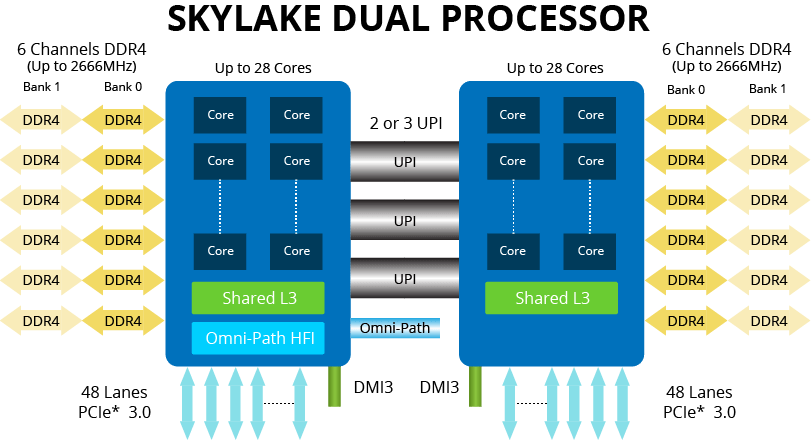
\includegraphics[width=10cm]{images/skylake_gold.png}
    \caption{\label{skylake_gold} Architecture d'une plate-forme avec deux processeurs Xeon Skylake (source \cite{Aspsys})}
\end{figure}



%%%%%%%%%%%%%%%%%
\subsubsection{Performances mémoire théoriques}
Le processeur Xeon Skylake 6148 possède 6 canaux mémoire pour accéder, dans notre expérimentation, à une mémoire DDR4-2666. En appliquant l'\autoref{eq:bw} nous obtenons une bande passante maximale de : $2666 \times 8 \times 6 = 128\ GB/s$. A cause de la loi de Little \cite{little2008little}, le processeur doit être capable de générer parallèlement suffisamment de chargement (\textit{outstanding load}) pour atteindre cette performance.


%%%%%%%%%%%%%%%%%
\subsubsection{Performances de calculs théoriques}
Le processeur étudié est un processeur superscalaire capable d'éxécuter jusqu'à 4 instructions par cycle dont deux opérations flottantes. Ces opération pouvant être des instruction FMA vectorielles de 512 bits. Il est donc possible de calculer sur chaque ALU, une multiplication et une addtion par cycle sur 8 éléments simultanément. On peut ainsi calculer la performances crête de ce processeur en appliquant l'\autoref{eq:flops}. Suivant la fréquence utilisable par le processeur (dépendant de la température) la performance crête théorique, $FLOPS_{peak}$ est comprise entre $8 \times 2 \times 2 \times 1.6 \times 20 = 1024\ GFLOP/s$ et  $8 \times 2 \times 2 \times 2.2 \times 20 = 1408\ GFLOP/s$. 

Cependant, pour comparer la performance de l'application avec ce résultat, il faut que la nature du code puisse utiliser des instructions FMA vectorisées. Il peut être intéressant de disposer d'une fourchette de performance lorsque la totalité du parallélisme est utilisé ou non. Quand le processeur n'utilisent pas d'instruction AVX-512, le processeur est capable d'atteindre 3.1 GHz lorsque les 20 coeurs sont actifs. En reprenant l'\autoref{eq:flops}, la performance optimale d'une telle application serait: $FLOPS_{SISD} = 1 \times 1 \times 2 \times 3.1 \times 20 = 124 \ GFLOP/s$.

%%%%%%%%%%%%%%%%%
\subsubsection{Équilibre arithmétique}
L'équilibre arithmétique du processeur permet d'évaluer s'il est approprié pour un code nécessitant une grande bande passante ou plutôt de bonnes performances de calculs. En réutilisant les deux caractéristiques précédemment calculées, on peut calculer $\text{EQUILIBRE}_{non\_avx}$ et $\text{EQUILIBRE}_{avx\_512}$ qui bornent la performances inférieure et supérieure de ce processeur. On obtient ainsi $\text{EQUILIBRE}_{non\_avx} = \frac{124}{128} = 0.97\ flop/byte$ et $EQUILIBRE_{avx\_512} = \frac{1408}{128} = 11\ \text{flopbyte}$. 
 

%%%%%%%%%%%%%%%%%
\subsubsection{L'efficacité énergétique}

La valeur  $EQUILIBRE_{avx\_512}$ est la plus pertinente des deux pour réaliser le choix de l'architecture. Les composants permettant de faire du calcul vectoriel sont compris dans le prix d'achat, qu'ils soient utilisés ou non. Si l'application portée est loin du ratio de 11 opérations flottantes pour 1 byte de données transféré, il faudra se tourner vers d'autres architecture, plus efficace. La notion d'efficacité se retrouve dans le ratio $flops/watt$.
\\
\textbf{tode}
\iffalse 
%%%%%%%%%%%%%%%%%%%%%%%%%%%%%%%%%%%%%%%%%%%%%%%%%%%%%%%%%%%%%%%%%%%%%%%%%%%%%%%%%%%%%%%%
%%%%%%%%%%%%%%%%%%%%%%%%%%%%%%%%%%%%%%%%%%%%%%%%%%%%%%%%%%%%%%%%%%%%%%%%%%%%%%%%%%%%%%%%
%%_______ .___________.    ___      .______    _______                      ___       %%
%%|   ____||           |   /   \     |   _  \  |   ____|                   |__ \      %%
%%|  |__   `---|  |----`  /  ^  \    |  |_)  | |  |__          ______         ) |     %%
%%|   __|      |  |      /  /_\  \   |   ___/  |   __|        |______|       / /      %%
%%|  |____     |  |     /  _____  \  |  |      |  |____                     / /_      %%
%%|_______|    |__|    /__/     \__\ | _|      |_______|                   |____|     %%
%%%%%%%%%%%%%%%%%%%%%%%%%%%%%%%%%%%%%%%%%%%%%%%%%%%%%%%%%%%%%%%%%%%%%%%%%%%%%%%%%%%%%%%%
%%%%%%%%%%%%%%%%%%%%%%%%%%%%%%%%%%%%%%%%%%%%%%%%%%%%%%%%%%%%%%%%%%%%%%%%%%%%%%%%%%%%%%%%
\fi


%%%%%%%%%%%%%%%%%%%%%%%%%%%%%%%%%%%%%%%%%%%%%%%%%%%%%%%%%%%%%%%%%%%
\section{Étape 2: Caractérisation des plate-formes}\label{sec:methodo_step2}
%%%%%%%%%%%%%%%%%%%%%%%%%%%%%%%%%%%%%%%%%%%%%%%%%%%%%%%%%%%%%%%%%%%

%%%%%%%%%%%%%%%%%
\subsection{Motivations et objectifs}
%%%%%%%%%%%%%%%%%

Pour pouvoir estimer la bonne ou mauvaise performance d'un code sur une plate-forme il est nécessaire de connaître la performance crête de cette dernière. Cette approche est utilisée par le modèle du \textit{roof line}. L'approche présentée dans cette thèse nécessite s'intéresse aux mêmes caractéristiques qui sont: la bande passante mémoire ($GB/s$) et la capacité calculatrice ($FLOP/s$). Il y a deux façons d'obtenir ces performances crêtes. La première méthode est de la calculer à partir des caractéristiques techniques de la plate-forme. Cette méthode à été utilisé lors de l'étape 1 permet de catégoriser les plate-formes qui pourront être envisagées pour porter l'application. La deuxième méthode est de la mesurer lors de l'exécution de l'application ou de benchmark. Pour la réalisation de cette étape, il faut avoir accès aux matériels pour pouvoir y réaliser les mesures. Des simulateurs peuvent aussi être utilisés bien que cette étape servent à mesurer les performances réelles de l'architecture.





%%%%%%%%%%%%%%%%%
\subsection{Mesure effective}
%%%%%%%%%%%%%%%%%
Une application industrielle peut être difficile à porter sur une nouvelle architecture dans le simple but de la caractériser. Il est préférable d'utiliser des benchmarks, plus court et plus facilement portable. Ces codes, souvent simple, permettent de caractériser une ou plusieurs parties d'une architecture. Cette valeur valeur est souvent inférieur à la performance théorique du fait de la complexité des architectures ou de la qualité du code généré. Par exemple pour mesurer la bande passante mémoire maximale atteignable on peut utiliser le benchmark \textit{Stream} \cite{McCalpin1995}, les latences des différents niveaux de caches \textit{lmbench} \cite{Staelin2002}. Pour mesurer le nombre maximum d'opération sur un nombre flottant exécutables par seconde, on peut utiliser le benchmark Linpack. 
L'avantage de cette approche est sa facilité. Il suffit de compiler le benchmark voulu et de l'exécuter pour obtenir les résultats. Si le code est optimale, cette méthode permet de mesurer la performance maximale réelle atteignable par l'architecture. Ainsi pourra comparer les performances de l'application avec les performances maximales atteignables par la plate-forme. 

L'inconvénient est que la mesure est dépendant de la qualité de code et du compilateur. Il peut arriver qu'en voulant mesurer spécifiquement un composant, les performances soient dégradées par une autre partie du sous système, empêchant ainsi la caractérisation exacte dont nous avons besoin. Par exemple, si l'on cherche à mesurer la bande passante maximale atteignable par un seul coeur avec un code simple lisant un tableau de données. Sur un processeur récent tel qu'un Xeon Skylake, on s'attendrait à obtenir une valeur proche du maximum théorique de 128 GB/s, calculé dans la partie précédente. Cependant, à cause de la Loi de Little \cite{little2008little} et de la taille de la queue de chargement (\textit{outstanding load queue}), il faut plus de dix coeurs actifs pour saturer la bande passante \cite{JohnMcCalpin2010}. Il faut donc une certaine expérience des outils et des micro-architectures pour apprécier les résultats mesurées. Il peut ainsi être nécessaire d'avoir plusieurs codes de benchmark à exécuter pour valider de différentes façon la micro-architecture. Nous avons développé un benchmark mémoire (section \ref{aaa}) et un benchmark de calcul (section \ref{bbbb}) pour générer différentes versions et évaluer une plate-forme le plus précisément possible.





%%%%%%%%%%%%%%%%%
\subsection{Application au processeur Intel Xeon 6148}
%%%%%%%%%%%%%%%%%
Nous mesurons les performances crête du bus mémoire, $\text{MEMORY}_{max}$ en GB/s, et du processeur $FLOP_{seconde\_max}$ en GFLOP/s, en utilisant deux contributions de la thèse: le benchmark mémoire \textit{dml\_mem} et le générateur de kernel, \textit{kernel\_generator}.


%%%%%%%%%%%%%%%%%
\subsubsection{Performances mémoires}


\textbf{Bande passante mesurée}
Nous utilisons le benchmark mémoire présenté dans \autoref{sec:dml}. A cause de la loi de Little \cite{little2008little}, nous utilisons la version MPI du benchmark sur les 20 coeurs pour s'assurer de saturer le bus mémoire grâce à la commande présentée dans \autoref{lst:dmlmem_xeon}. Nous obtenons une bande passante mémoire $\text{MEMORY}_{max}$ de 105 GB/s que nous avons vérifié avec l'outil \textit{YAMB}.\\

\begin{lstlisting}[caption=Commande utilisée pour obtenir la bande passante maximale avec le benchmark \textit{DML\_MEM}, label={lst:dmlmem_xeon},
  basicstyle=\footnotesize, frame=tb,
  xleftmargin=.065\textwidth, xrightmargin=.065\textwidth]
mpirun -np 20 numactl dml_mem  --steplog 0 --unroll 8 
       --type read --stride 64 --matrixsize 5000
\end{lstlisting}


%%%%%%%%%%%%%%%%%
\subsubsection{Performance de calculs}


\textbf{Performance de calculs mesurée}: nous utilisons le générateur de benchmark \textit{Kernel\_Generator} (voir \autoref{seq:kg}) pour évaluer le nombre maximum d'opérations FMA AVX-512 réalisable sur un nombre flottant à double précision. Pour cela nous avons utilisé la commande présentée dans l'\autoref{code:kg_512}. Nous générons un kernel de 14 instructions FMA pour réduire le coût de gestion de la boucle (incrémentation et comparaison) et masquer la latence des instructions.\\

\begin{lstlisting}[caption=Commande utilisée pour obtenir la performance crête du processeur (GFLOP/s) avec le générateur de benchmark \textit{Kernel\_Generator}., label={code:kg_512},
  basicstyle=\footnotesize, frame=tb,
  xleftmargin=.065\textwidth, xrightmargin=.065\textwidth]
./kg -W 512 -O ffffffffffffff -P double -S 100 -L 120000000
\end{lstlisting}


Le benchmark généré ne possède pas de version multi-coeurs, nous lançons donc indépendamment 20 exécutions du binaire que l'on accroche à un coeur différent grâce à un paramètre du benchmark. Pour cette expérience nous avons commencé par désactiver le turbo du processeur, et limité sa fréquence à 1.6GHz. La performance mesurée est de 998.57 GFLOP/s. Ensuite nous avons activé le turbo, et laissé le processeur choisir lui même sa fréquence. L'\autoref{code:kg_512_output} montre les résultats donnés par le benchmark pour l'exécution sur un des 20 coeurs. Le benchmark mesure sa fréquence effective et trouve bien la valeur de 2.2 GHz renseigné par Intel dans sa documentation. La performance crête d'un coeur est de 69.2 GFLOP/s, approchant le maximum théorique de 70 GFlop/s.


\begin{lstlisting}[caption=Résultat de l'exécution du benchmark sur un coeur avec le turbo activé, label={code:kg_512_output},
  basicstyle=\footnotesize, frame=tb,
  xleftmargin=.005\textwidth, xrightmargin=.005\textwidth]
------------------  INSTRUCTIONS SUMMARY ------------------------------
_label_|   NB INSTRUCTIONS      Time    FREQUENCY    inst/sec       IPC
_value_|      168000000000      38.8          2.2     4.33e+9      2.01
----------------------  FLOP SUMMARY  ---------------------------------
 PRECISION     FLOP/cycle         FLOP/second
    Single              0                   0
    Double           32.0            6.92e+10
-----------------------------------------------------------------------
\end{lstlisting}

Pour vérifier que les 20 coeurs effectuaient bien le même travail, un outil de profilage développé en interne, appelé \textit{mygflops.sh}, a été utilisé. Il permet de compter les instructions flottantes simple et double précision exécutées sur un processeur. Le résultat est présenté dans l'\autoref{code:mygflops_512_output}. La performance crête mesurée du processeur est de 1372.78 GFlop/s, proche du maximum théorique calculé précédemment de 1408 GFLOP/s.

\begin{lstlisting}[caption=Résultat de l'outil \textit{myflops.sh} utilisé pour compter les instructions flottante exécutées sur un processeur., label={code:mygflops_512_output},
  basicstyle=\footnotesize, frame=tb,
  xleftmargin=.005\textwidth, xrightmargin=.005\textwidth]
Single-precision SSE/AVX :       0.00 GFlop/s  --   0.0% of Flops
Double-precision SSE/AVX :     (*\bfseries 1372.78 GFlop/s*)  -- 100.0% of Flops
   0.0% scalar  64-bit SSE/AVX instructions (  0.0% of fp instructions)
   0.0% packed 128-bit SSE/AVX instructions (  0.0% of fp instructions)
   0.0% packed 256-bit AVX instructions     (  0.0% of fp instructions)
 100.0% packed 512-bit AVX instructions     (100.0% of fp instructions)
\end{lstlisting}
%%%%%%%%%%%%%%%%%%%%%%%%%%%%%%%%%%%%%%%%%%%%%%%%%%%%%%%%%%%%%%%%%%%
\section{Étape 3: Extraction de noyaux et modélisation de leur performance} \label{sec:methodo_step3}
%%%%%%%%%%%%%%%%%%%%%%%%%%%%%%%%%%%%%%%%%%%%%%%%%%%%%%%%%%%%%%%%%%%

Les deux premières étapes de la méthodologie s'intéressent à la recherche et à la caractérisation de nouvelles plateformes. La troisième étape peut être réalisée en parallèle et concerne la modélisation des performances de l'application.


%%%%%%%%%%%%%%%%%
\subsection{Motivations et objectifs}
%%%%%%%%%%%%%%%%%


    En introduction de cette partie, nous avons rappelé la définition des noyaux (\textit{hot spots}). Ceux-ci sont particulièrement présents dans les applications de calcul haute performance qui peut en posséder plusieurs. Ces zones de codes possèdent un fort potentiel pour l'amélioration de la performance de l'application.  Si une application passe 99\% de ses cycles dans l'exécution d'une fonction, une amélioration d'un facteur 10 de celle-ci entraînera une amélioration du même facteur de l'application. Le travail du programmeur est donc d'identifier et d'accélérer ces parties en priorité.
    
    Les applications réelles utilisées en production dépassent souvent les dizaines de milliers de lignes de codes. Porter et optimiser la totalité d'une application serait complexe et contre-productif. De plus, chaque noyau pouvant avoir des besoins différents (\textit{memory bound} ou \textit{compute bound}), il est nécessaire de les porter individuellement sur différentes plateformes. 
    
    L'objectif de cette étape est d'identifier ces zones du code clés et de modéliser leur performance en fonction des performances de la bande passante mémoire (GB/s) ou du processeur (FLOP/s) en calculant leur intensité opérationnelle $\text{OI}_{noyau}$. La majorité des codes étant limité par la performance de la mémoire, la thèse présente un modèle de performance basé sur ces performances. 


%%%%%%%%%%%%%%%%%
\subsection{Identification des noyaux}
%%%%%%%%%%%%%%%%%
    
    
    De nombreux travaux sont réalisés pour identifier et extraire les noyaux d'une application \cite{castro2015cere, brunst2013custom}. L'outil de profilage \textit{perf} \cite{de2010new} permet d'extraire un sommaire de l'exécution d'une application en représentant son arbre d'appel (voir \autoref{perf_example}). 
    


\begin{lstlisting}[caption=Exemple d'utilisation de l'out perf avec la commande \textit{perf record  -g  -F 97}. Le rapport d'exécution est obtenu avec la commande \textit{perf report --stdio}, float,floatplacement=H, label={perf_example}]
# Samples: 116K of event 'cycles:ppp'
# Event count (approx.): 2744862582690
#
# Children      Self  Command          Shared Object       Symbol                                                                       
# ........  ........  ...............  .................. .......
    99.52%     0.00%  Stream.SKL.128   [unknown]           [k] 0000000000000000
            |          
             --99.52%--0
                       |          
                        --99.16%--0xadf96
                                  |
                                  |--25.35%--tuned_STREAM_Add   
                                  |--25.34%--tuned_STREAM_Triad
                                  |--20.36%--tuned_STREAM_Copy
                                  |--17.27%--tuned_STREAM_Scale
                                   --10.74%--main

\end{lstlisting}



%%%%%%%%%%%%%%%%%
\subsection{Modélisation de l'équilibre des noyaux}
%%%%%%%%%%%%%%%%%
    
    Chaque noyau peut être porté sur un accélérateur différent, et leur analyse doit se faire indépendamment les uns des autres. L'objectif de la modélisation est de comprendre les performances de l'application: si elles limitées par les performances du système mémoire ou par la capacité de calcul du processeur. La modélisation des performances permet de réduire le nombre de plateformes envisagées pour le portage de l'application. Cette étape permet d'éviter d'investir du temps et de l'argent dans des solutions inefficaces pour l'application étudiée. 
    
 
 \textbf{TODO check ça y a un char en trop ?}   
%    Pour cela, le \textit{Roofline Model}, permet de réaliser cette représentation des performances. Il est présenté dans la \autoref{sec:Roofline}. Nous conseillons de construire le modèle à l'aide des caractéristiques mesurées lors de l'étape 2 ($\text{PERF_{peak}}$) pour avoir une meilleure estimation des performances réellement atteignables. 
    Il est nécessaire de calculer l'intensité opérationnelle, $\text{OI}_{noyau}$, mesurée en $flop/byte$. Elle représente le nombre d'opérations réalisables par le processeur pour chaque donnée transférée depuis la mémoire. Ce calcul se fait à partir de la lecture de code source, motivant le besoin d'identifier individuellement les noyaux de calculs. 
    L'utilisation du modèle permet ensuite de visualiser les noyaux ayant le plus grand potentiel d'amélioration de performance. 


%%%%%%%%%%%%%%%%%
\subsection{Simple Memory Model: Modélisation de la performance mémoire} \label{sec:smm}
%%%%%%%%%%%%%%%%%

    La majorité des codes HPC exécutée sur des architectures modernes voient leurs performances limitées par celle de la bande passante mémoire. Nous avons développé un modèle de performance simple, permettant de modéliser et valider les performances d'un code facilement. Pour réaliser cette modélisation, le développeur doit avoir accès au code source de l'application à porter. Pour un noyau donné, il faut compter le nombre d'accès mémoire en distinguant les accès en lecture et ceux en écriture. Il est important de distinguer les accès en lecture et en écriture, car nous utiliserons leur ratio pour valider le bon comportement de la microarchitecture avec l'outil YAMB. En effet, nous montrons dans notre expérience que la saturation du bus mémoire n'est pas un indicateur suffisant pour conclure de l'efficacité ou non d'un code.
    
    Cette modélisation est faisable seulement si les noyaux du code ont été identifiés, l'appliquer sur la totalité de l'application serait trop long. Si la taille des jeux de données $\text{DATA}_{size}$ est connue, il est alors possible de calculer la quantité de données minimale qui doit être transférée sur le bus mémoire. Grâce à l'étape 2, nous connaissons les performances maximales théorique $\text{MEMORY}_{peak}$ et réelle $\text{MEMORY}_{max}$ de la microarchitecture. Il est donc possible de calculer la durée optimale pour exécuter fonction étudiée, $\text{TEMPS}_{optimal}$, mesurée en seconde. Le modèle assume que le code utilise un algorithme parfait (utilisation de la localité des données), que sa compilation du code à été réalisée avec un compilateur parfait et qu'il est exécuté sur une plateforme parfaite. L'objectif n'est pas d'atteindre exactement cette performance, mais de s'en approcher le plus possible. Généralement, lorsqu'un défaut apparaît à un des niveaux énumérés précédemment, la performance s'éloigne radicalement de la performance optimale.
    
    \begin{equation}
        \text{TEMPS}_{optimal}\ = \frac{\text{DATA}_{size}}{\text{MEMORY}_{max}}
    \end{equation}





%%%%%%%%%%%%%%%%%
\subsection{Application des modèles Roofline et SMM au benchmark Stream}
%%%%%%%%%%%%%%%%%
    
    L'\autoref{perf_example} montre le profil de l'exécution du benchmark \textit{Stream}. Il comporte quatre fonctions utilisées pour stresser la mémoire par différent type d'accès. Nous choisissons arbitrairement de consacrer notre analyse sur un des quatre noyaux de Stream: la fonction \textit{triad} dont le code peut être vu dans l'\autoref{code:triad}. Cette fonction est intéressante, car ce motif d'accès est très courant dans les applications HPC.
    
    
\begin{lstlisting}[language=c,caption= La fonction triad du benchmark Stream utilise trois matrices: deux en lecture et une en écriture,label={code:triad}, 
  basicstyle=\footnotesize, frame=tb,
  xleftmargin=.065\textwidth, xrightmargin=.065\textwidth]
for (j=0; j < STREAM_ARRAY_SIZE; j++)
    A[j] = B[j] + scalar * C[j];
\end{lstlisting}
        
        
    
    \subsubsection{Modèle du Roofline}
    %%%%%%%%%%%%%%%%%
        Lors de l'étape 1, nous avons mesuré la performance mémoire maximale atteignable $\text{MEMORY}_{max}$ de 105 GB/s. L'utilisation du \verb|Kernel Generator| nous avait permis de mesurer une performance $\text{FLOPS}_{max}$ de 1372.78 GFlop/s, proche de la performance théorique de l'architecture. Ces deux mesures permettent de construire le \textit{toit} du modèle du Roofline présenté sur la \autoref{pic:Roofline_stream}.
        
        Pour étudier les limitations du noyau étudié, il est ensuite nécessaire de calculer son intensité opérationnelle. Lors de chaque itération de boucle, le processeur doit charger 3 éléments en double précision, soit 24 bytes. En effet, or optimisation, une ligne de cache doit être chargée avant d'être écrite, même si aucune des données n'est utilisée en lecture par le processeur. À chaque itération de boucle, deux opérations doivent être réalisées, une addition et une multiplication. Cette fonction a donc une intensité arithmétique $\text{OI}_{noyau} = \frac{2}{24} = 0.083\ flop/byte$.
        Pour comparaison, les processeurs récents ont un ratio proche de $10\ flop/byte$. Cette simple modélisation montre le déséquilibre qu'il y a entre la performance de la mémoire et celle des processeurs. Elle permet de guider le choix de la plateforme sur laquelle cette fonction devra être portée. La \autoref{pic:Roofline_stream} montre l'application du Roofline à l'étude de la fonction triadd et au processeur étudié. Cette fonction ayant un faible $\text{OI}_{noyau}$, ses performances théoriques mesurées en flop sont elles aussi très faibles.
        
        \begin{figure}
            \center
            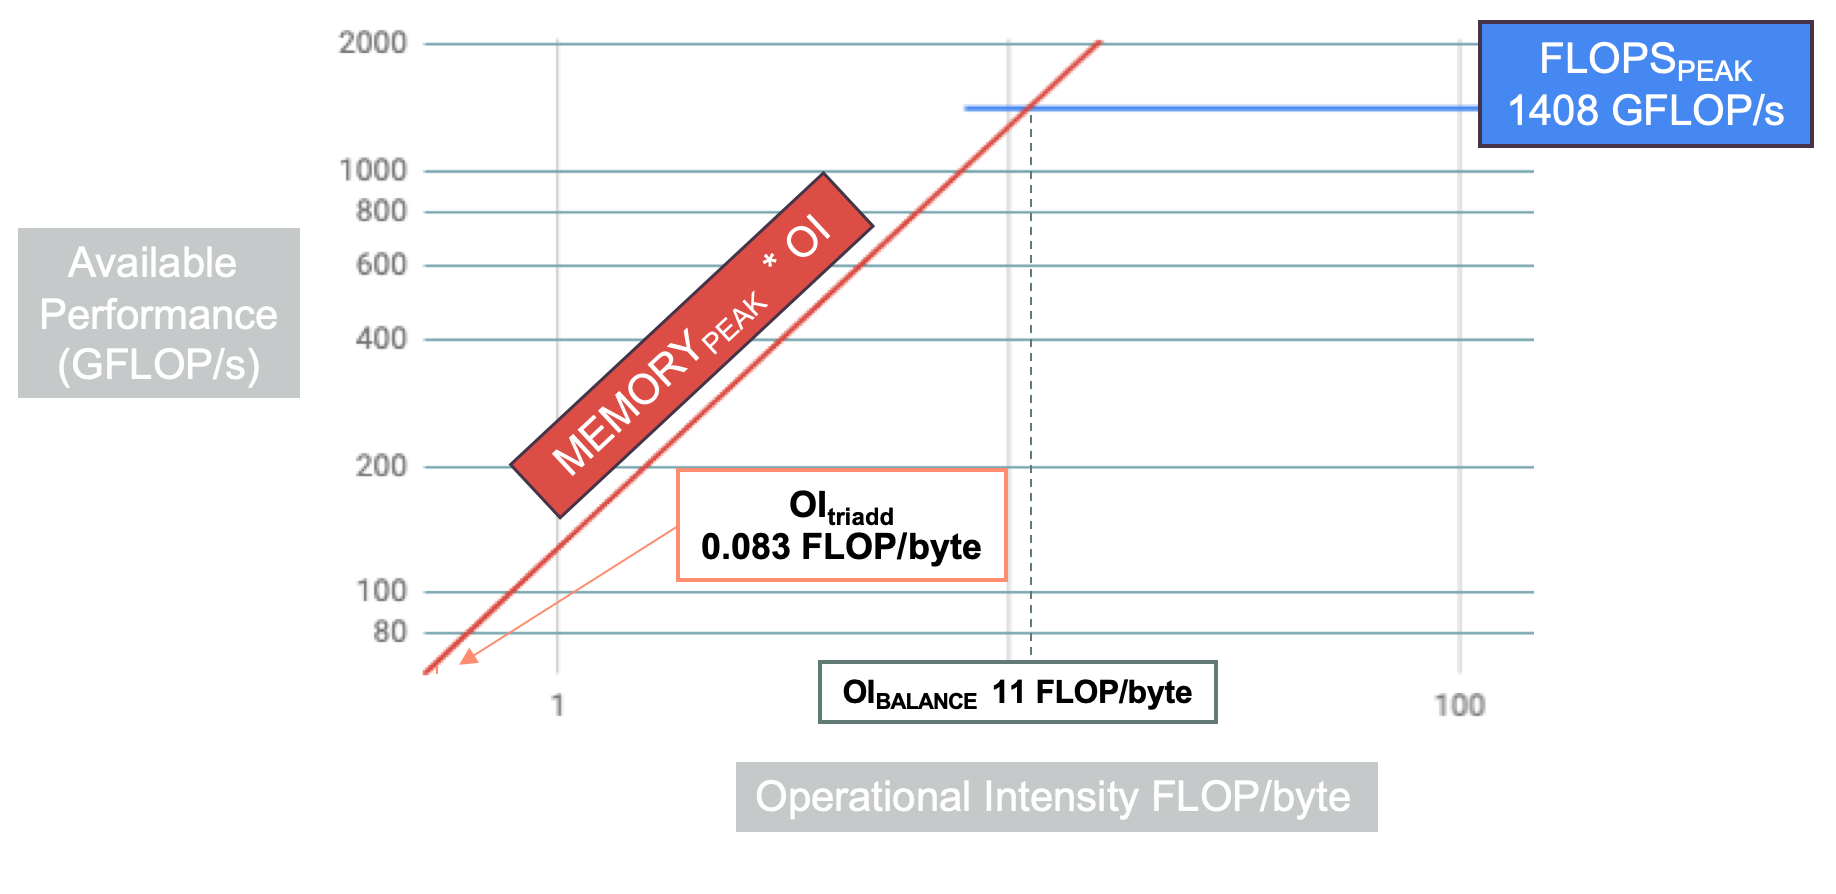
\includegraphics[width=14cm]{images/roofline_stream.png}
            \caption{\label{pic:Roofline_stream} Modèle du \textit{Roofline} appliqué à la fonction \textit{triadd} du benchmark \textit{Stream} et un processeur Xeon Skylake 6148.}
        \end{figure}
    


\subsubsection{Simple Memory Model} 
%%%%%%%%%%%%%%%%%
    L'analyse du noyau avec le modèle du Roofline indique que sur l'architecture ciblée, la performance du code sera limitée par la performance de la bande passante.

    
    Une fois assuré que les performances de l'application sont limitées par le système mémoire, le Simple Memory Model peut être appliqué. Dans notre expérimentation, nous utilisons trois matrices de 19.6 GB ($3 \times 10^9 \times sizeof(double)$). Pour une exécution optimale, le bus mémoire devrait être utilisé pour charger une fois les deux matrices en lectures (matrices B et C)  et pour l'écriture de la matrice A. Le trafic mémoire total serait alors de 58.8 GB. En utilisant les résultats mesurés lors de l'étape 2, on peut estimer le temps optimal pour l'exécution de cette fonction: $\text{TEMPS}_{optimal} = \frac{58.8}{128} = 0.56$ seconde. Cette modélisation nous permet de projeter la performance optimale sur une architecture sans avoir à exécuter le code sur celle-ci. Ainsi, nous pouvons comparer cette valeur avec la performance de l'architecture actuellement utilisée. Ceci permet de quantifier le gain de performance et d'avoir un modèle de performance à vérifier lorsque le portage sera réalisé.
%%%%%%%%%%%%%%%%%%%%%%%%%%%%%%%%%%%%%%%%%%%%%%%%%%%%%%%%%%%%%%%%%%%
\section{Étape 4: Sélectionner la plateforme adaptée} \label{sec:methodo_step4}
%%%%%%%%%%%%%%%%%%%%%%%%%%%%%%%%%%%%%%%%%%%%%%%%%%%%%%%%%%%%%%%%%%%


    Les deux premières étapes ont permis de trouver et de caractériser de potentielles architectures. À l'aide de plusieurs benchmarks, certaines caractéristiques clés des architectures ont pu être obtenues. Lors de l'étape 3, l'extraction et la modélisation des \glspl{hotspot} ont été faites.  Cette quatrième étape consiste à réaliser le choix de l'architecture la plus adaptée pour l'exécution de chaque hot spot. Ce choix est réalisé en prenant en considération la performance des architectures, les besoins de l'application étudiée ainsi que d'autres critères (voir \autoref{pic:methodo_step4}).
    
    \begin{figure}
        \center
        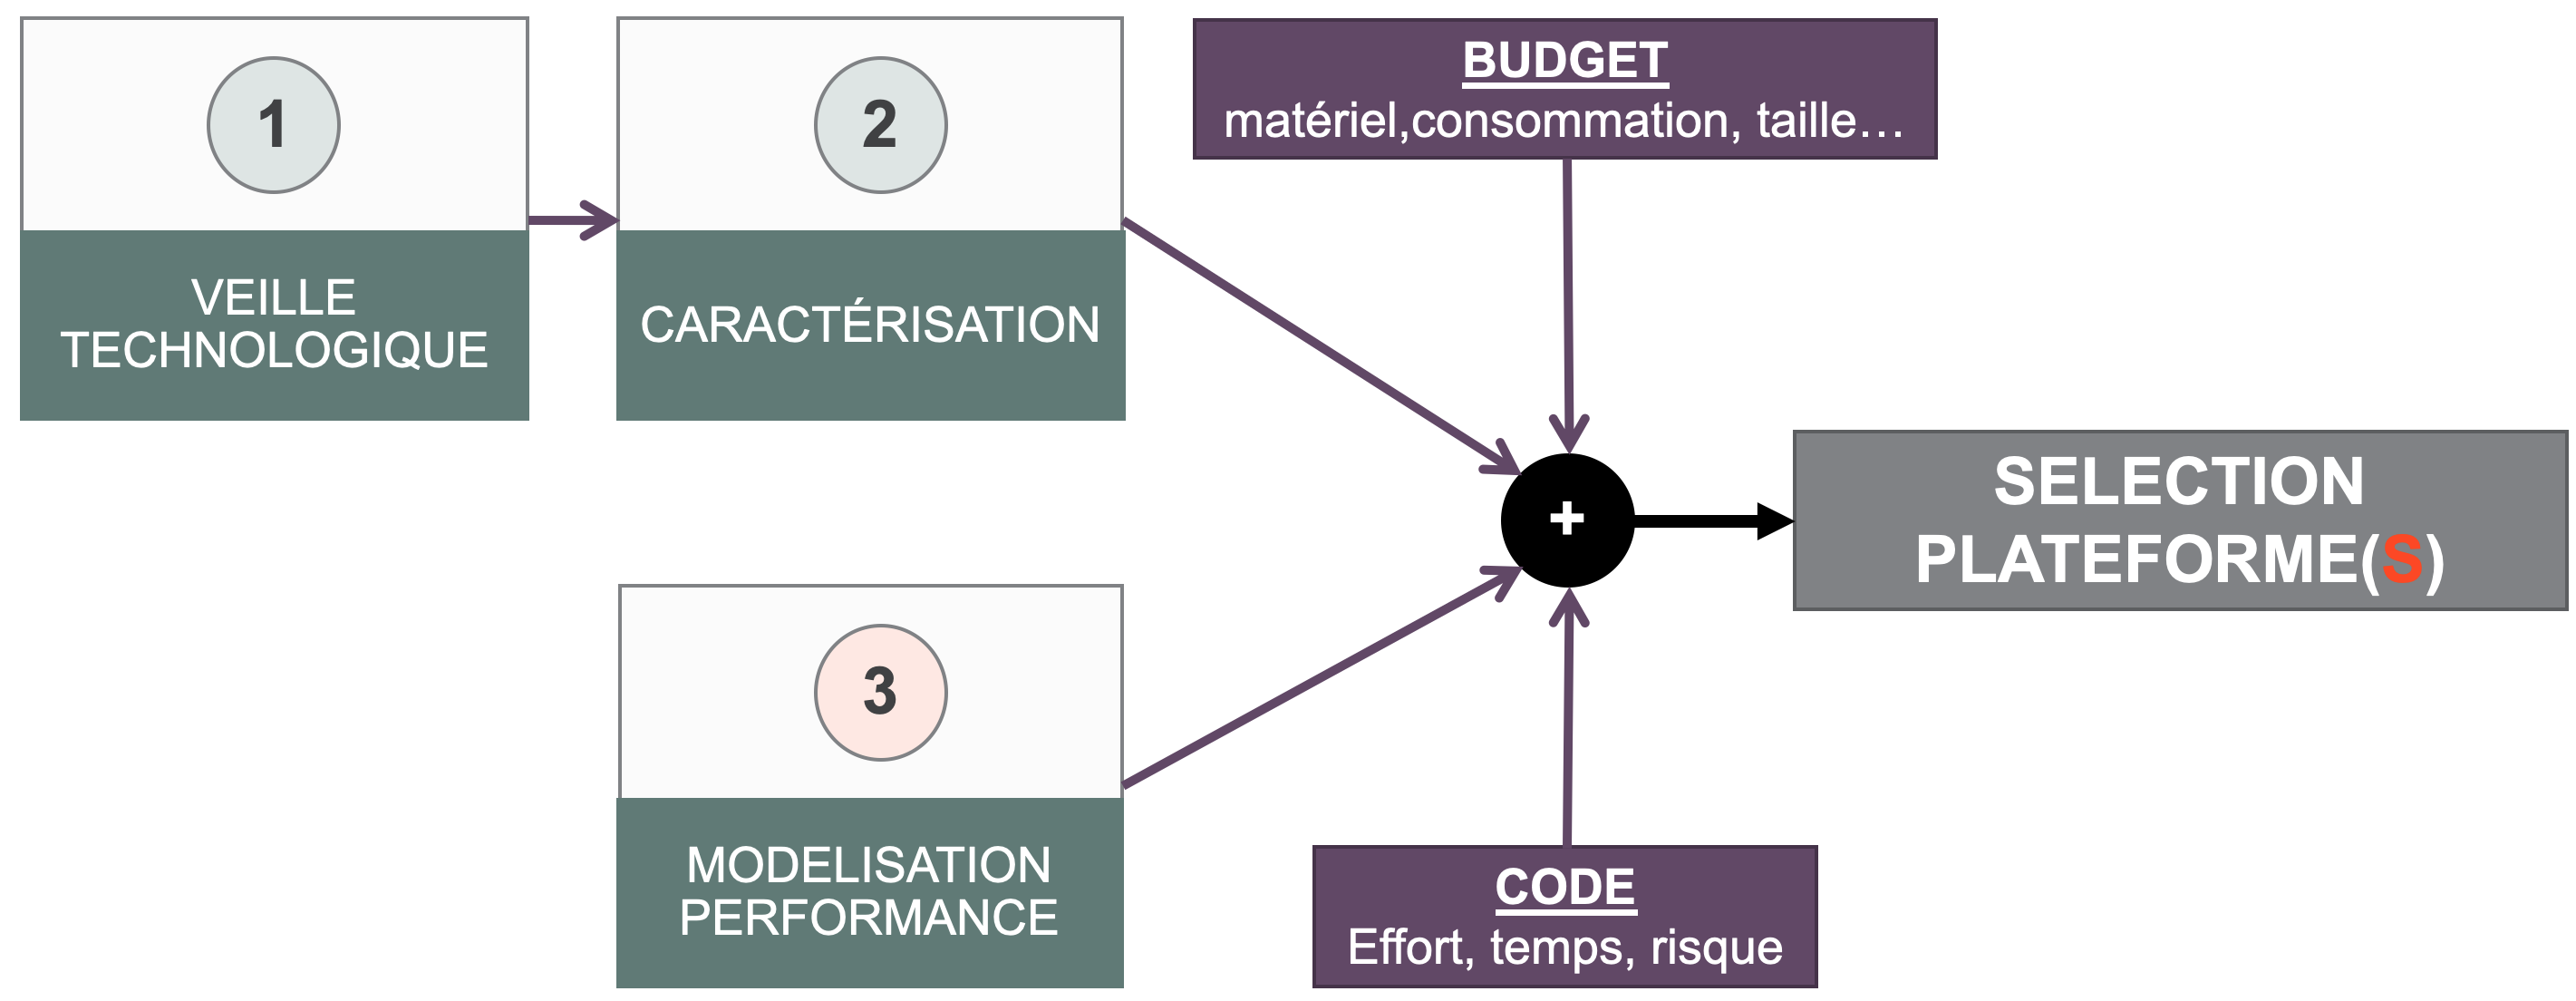
\includegraphics[width=14cm]{images/methodo_step4.png}
        \caption{\label{pic:methodo_step4}L'étape 4 consiste à choisir les plateformes adaptées aux différents noyaux en fonction de plusieurs critères.}
    \end{figure}



%%%%%%%%%%%%%%%%%
\subsection{Le coût}
%%%%%%%%%%%%%%%%%
    
   Le prix des architectures est un élément important pour choisir la ou les architectures utilisées pour la construction de la plateforme. Cependant, utiliser le prix unitaire des accélérateurs choisis n'est pas suffisant et il est nécessaire de prendre en compte d'autres paramètres dans le calcul du prix appelé coût total de possession (TCO). Il prend en compte tous les coûts engendrés par le centre de données durant son cycle de vie: construction des bâtiments, consommation électrique, etc.
   %Le budget pour la construction du premier centre exascale européen est de 500 millions d'euros \cite{SergiGirona2018}.
    
    \paragraph{Le prix du matériel} 
        Le  prix des accélérateurs et du matériel nécessaires à la construction du supercalculateur constituent une part significative dans le calcul du coût. En fonction du prix de l'accélérateur, une solution moins performante pourra lui être préférée. Les cartes FPGA sont un bon exemple d'architectures très performantes, mais peu utilisées dans les supercalculateurs. Bien que la complexité de programmation y participe, le prix des cartes FPGA est une raison majeure de leur faible utilisation dans les plateformes modernes.
    
    \paragraph{La consommation électrique}
        La consommation électrique de la plateforme finale est devenue un critère très important dans le choix du matériel. La consommation des centres de données est un réel investissement qui doit être mesuré et anticipé lors de l'achat du matériel. Un supercalculateur consommant 10 MW engendrera une facture de plusieurs millions d'euros chaque année. Le prix de l'électricité et l'enveloppe énergétique disponible pour le calcul varient avec l'emplacement choisi pour installer le centre de calcul. La majorité des centres ayant des lignes électriques déjà construites ne peuvent acheminer qu'une quantité limitée de courant. L'enveloppe énergétique disponible est alors une contrainte forte pouvant favoriser l'utilisation d'une architecture plus efficace énergétiquement.
        
        En comparant  l'intensité opérationnelle d'un kernel (\gls{oikernel}) et l'équilibre arithmétique de l'architecture (\gls{equilibrearchi}) il est possible d'estimer la pertinence d'un accélérateur pour un noyau. Des valeurs proches indiquent que l'architecture ciblée est adaptée au code étudié et que l'accélérateur choisi aura un meilleur rendement énergétique. Un code faisant peu de calculs flottants ne nécessitera pas l'utilisation de coeurs complexes réalisant plusieurs dizaines de \gls{FLOP} par cycle. Bien que non utilisés, ces composants impactent le prix de la solution, mais aussi sa consommation électrique. 
        
                %La chaleur de la zone géographique de son installation impactant le refroidissement nécessaire. Ainsi en 2018, Microsoft a décidé de couler ses serveurs au fond de l'océan pour profiter d'un refroidissement gratuit \cite{ChristineHall2018}.
            
    \paragraph{La taille du centre de données} 
        Souvent les centres de données sont déjà existants et la taille disponible pour la création d'un supercalculateur ou l'ajout de nouveaux serveurs est une contrainte forte. Certaines solutions prenant plus ou moins de place pour être installées, le ratio $\frac{flop}{m^2}$ peut alors être calculé pour évaluer la densité des serveurs pour s'adapter aux contraintes du lieu. Si le bâtiment doit être construit pour accueillir le supercalculateur, son coût doit entrer dans le calcul de la solution finale.




%%%%%%%%%%%%%%%%%
\subsection{La performance}
%%%%%%%%%%%%%%% \cite{Rodero2012}%%
    D'autres critères concernant la performance et l'optimisation du code doivent être pris en compte pour choisir la ou les architectures utilisées pour accélérer l'exécution de l'application.
    
    \paragraph{Performance du noyau}
        Bien sûr, le gain de performance obtenu après le portage d'un \gls{kernel} sur un accélérateur est un critère important.
        La performance du noyau a un impact financier, car s'il est exécuté plus rapidement, d'autres applications pourront alors accéder à la plateforme. Les clients de supercalculateurs ont généralement un budget fixe et de multiples applications à exécuter. Ils cherchent alors à optimiser l'utilisation des ressources informatiques par les différents codes. Bien que l'on considère qu'il est nécessaire de porter individuellement chaque noyau sur l'accélérateur le plus adapté, il faut aussi prendre en considération le reste de l'application, mais aussi les applications des autres utilisateurs. Si une seule des applications ne bénéficie pas des performances d'un accélérateur, il serait plus pertinent d'opter pour un accélérateur adapté à plusieurs applications exécutées sur la plateforme. 
    
     
    \paragraph{Difficulté du portage}
        Les transformations de codes nécessaires pour porter le code d'un kernel sur une architecture doivent être évaluées. Celles-ci peuvent avoir un impact sur les performances finales (incapacité à réaliser les optimisations nécessaires) ou sur le coût (recours à des programmeurs expérimentés).  Suivant l'architecture choisie, il faudra peut-être coder l'application avec un nouveau langage, utiliser de nouvelles librairies ou de nouveaux modèles de programmation. Lorsque l'implémentation d'une optimisation est décidée, le risque de ne pas parvenir à obtenir les performances espérées doit lui aussi être mesuré. Le temps optimal, noté \gls{tempsoptimal}, pour exécuter l'application considère que l'application utilise de façon optimale l'architecture. Cependant pour atteindre ces performances, le noyau peut nécessiter l’utilisation d'optimisations complexes, pouvant être difficile à implémenter sur des applications industrielles. Il peut arriver qu'une optimisation moins performante soit préférée, car la transformation du code est plus facile. Le temps et le nombre de programmeurs nécessaires à son implémentation entrent alors aussi en considération dans le prix de la solution.
    
                           
%%%%%%%%%%%%%%%%%%%%%%%%%%%%%%%%%%%%%%%%%%%%%%%%%%%%%%%%%%%%%%%%%%%
\section{Étape 5: Portage et optimisation du code} \label{sec:methodo_step5}
%%%%%%%%%%%%%%%%%%%%%%%%%%%%%%%%%%%%%%%%%%%%%%%%%%%%%%%%%%%%%%%%%%%

Lors de l'étape 4, une plateforme a été choisie en fonction de plusieurs critère pour y porter les noyaux. L'étape 5 s'occupe du portage du code et de la validation du modèle de performance. 


%%%%%%%%%%%%%%%%%
\subsection{Introduction}
%%%%%%%%%%%%%%%%%

    \subsubsection{Motivations}
    %%%%%%%%%%%%%%%%%%%%%%%%%%%%%%
    Une fois le choix de la plateforme adaptée au noyau dans l'étape 4, le travail de portage doit être réalisé. 
    Une difficulté rencontrée par le programmeur est de s'assurer que les performances obtenues après le portage sont celles attendues par les prédictions. L'utilisation d'une nouvelle plateforme apporte une difficulté supplémentaire concernant la compatibilité des outils. Le programmeur doit alors être capable de poursuivre son analyse de performance avec des outils simples. 
    L'objectif de cette étape est de montrer au programmeur comment les outils présentés dans cette thèse, peuvent l'aider à valider la performance du noyau établie lors de l'étape 3.

    
    \subsubsection{Premier développement}
    %%%%%%%%%%%%%%%%%
        Une fois la plateforme choisie il faut appliquer les transformations du code nécessaires pour pouvoir y exécuter les noyaux. L'effort nécessaire pour adapter le code à cette nouvelle architecture a dû être évalué lors de l'étape précédente. Le portage du code peut nécessiter un changement de langage de programmation ou de paradigme de programmation.
        Si possible, il est important d'utiliser des librairies déjà optimisées pour espérer atteindre les performances crêtes de l'application. De plus, les constructeurs de la plateforme peuvent avoir développé des librairies pouvant être quasi-optimales et qui nécessitent une grande expertise pour être développées.
        
        Pour atteindre le maximum de performance, le code doit profiter au maximum de la parallélisation. Pour cela, le maximum de coeurs doivent être utilisés, grâce aux paradigmes de programmation partagée et distribuée. Les processeurs étant généralement superscalaires (voir \autoref{sec:superscalar}) il faut essayer d'exécuter le maximum d'instructions chaque cycle. Le dernier niveau de parallélisme est apporté par l'utilisation d'instructions vectorielles. Lorsque c'est possible des instructions telles que les FMA doivent être utilisées. Les différentes pistes listées peuvent nécessiter l'utilisation d'un simple drapeau lors de la compilation ou au contraire nécessiter de lourdes modifications du code et des jeux de données.
    

\subsection{Analyse de performance}
%%%%%%%%%%%%%%%%%

    Lors de l'étape 4, un modèle de performance du noyau a été établi (voir paragraphe \ref{sec:smm}). Une fois porté sur la nouvelle plateforme, il convient de vérifier les performances obtenues. La \autoref{pic:methodo_step5} propose un cheminement à suivre pour la validation et l'optimisation des performances.

\begin{figure}[h!]
    \center
    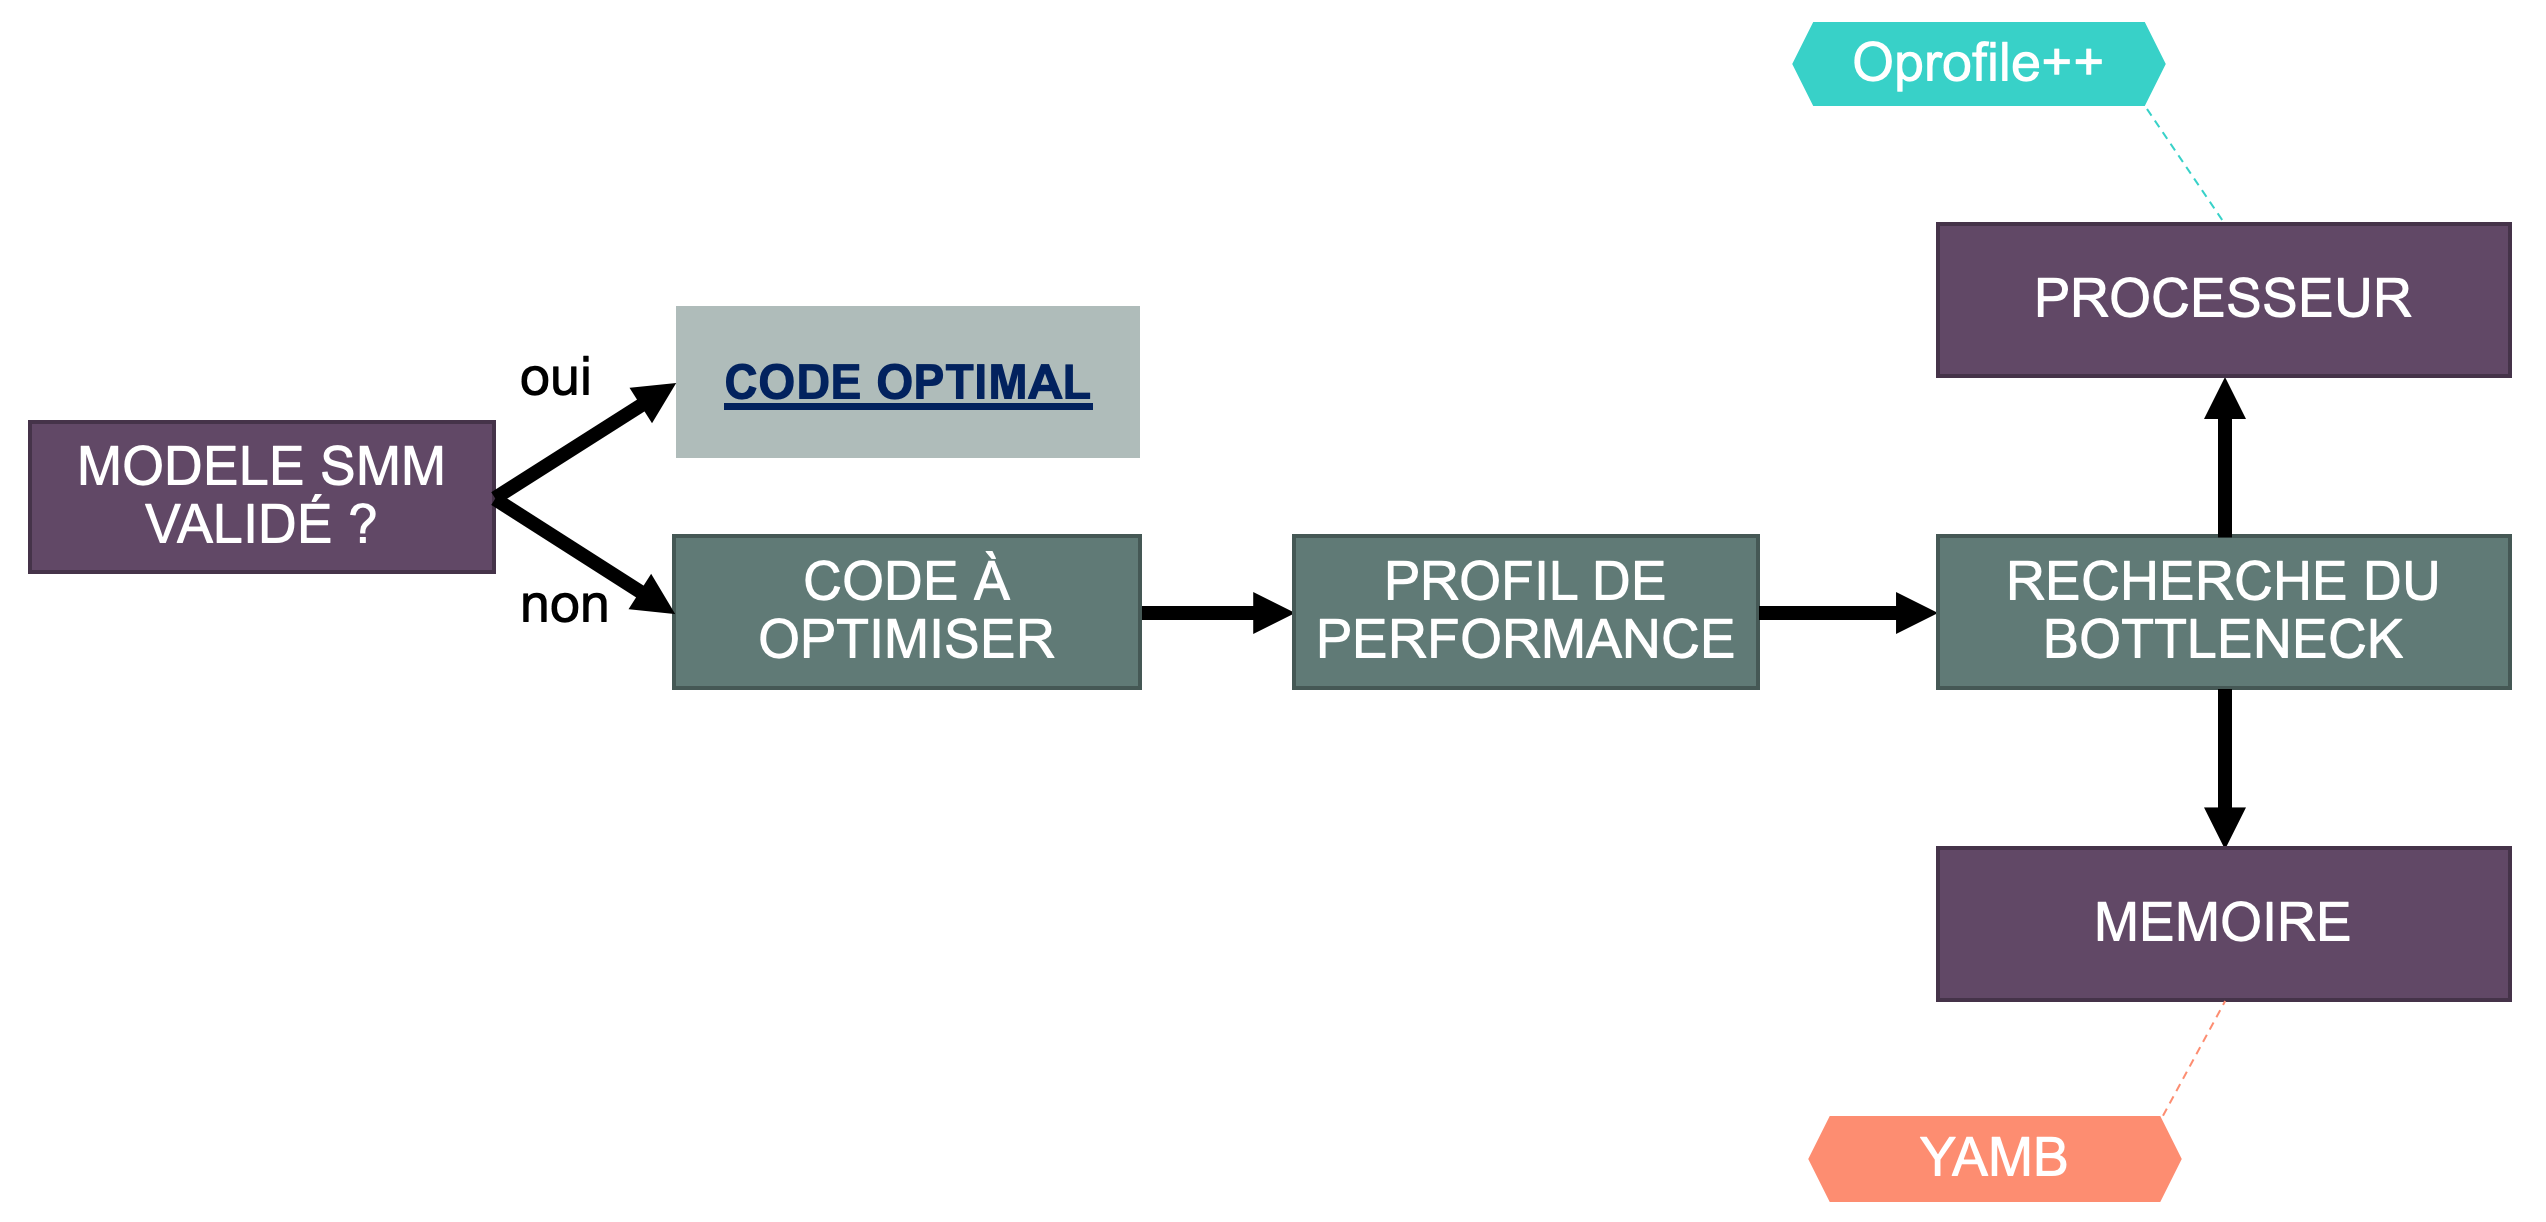
\includegraphics[width=14cm]{images/methodo_step5.png}
    \caption{\label{pic:methodo_step5}Les différentes étapes à suivre pour valider la performance du noyau.}
\end{figure}




    \subsubsection{Vérification du modèle de performance}
    %%%%%%%%%%%%%%%%%
    
        La première étape de l'analyse est de valider que la performance atteinte par le code est proche de celle calculée par notre modèle SMM. Dans le cas contraire, cela permet de quantifier l'écart par rapport à l'optimum théorique $\text{TEMPS}_{optimal}$. 
        
        Pour mesurer le temps d'exécution du noyau, $\text{TEMPS}_{mesure}$, nous proposons d'utiliser la fonction \textit{gettimeofday ()} \cite{Linux}. Cette fonction est disponible sur la totalité des systèmes Linux et permet de récupérer l'heure actuelle avec une précision allant jusqu'à la microseconde. Le but de la méthodologie présentée est de porter les codes sur de nouvelles architectures. Baser l'analyse de performance sur des compteurs matériels trop complexes aurait réduit la portabilité de notre démarche. On peut mesurer  $\text{TEMPS}_{mesure}$ en plaçant deux appels à la fonction \textit{gettime} présentée dans l'\autoref{lst:gettime}, avant et après le noyau.
        
        
        \begin{lstlisting}[language=c,caption=Fonction utilisée pour lire la date actuelle avec une précision allant jusqu'à la microseconde,label={lst:gettime}, 
          basicstyle=\footnotesize, frame=tb,
          xleftmargin=.065\textwidth, xrightmargin=.065\textwidth]
        double gettime()
        {
          struct timeval tp;
          struct timezone tzp;
          int i;
          i = gettimeofday(&tp,&tzp);
          return ( (double) tp.tv_sec + (double) tp.tv_usec * 1.e-6 );
        }
        \end{lstlisting}
        
        Si $\text{TEMPS}_{mesure}$ est proche de $\text{TEMPS}_{optimal}$ alors le noyau est proche d'avoir des performances optimales. Dans le cas contraire, l'analyse de performance doit se poursuivre pour en connaître la cause. La mesure $\text{TEMPS}_{optimal}$ permet d'avoir un objectif de performances à atteindre et de savoir quand le travail d'optimisation est terminé.
        
    
    \subsubsection{Profilage des performances}
    %%%%%%%%%%%%%%%%%

        Si la mesure de $\text{TEMPS}_{mesure}$ est inférieur à l'optimale $\text{TEMPS}_{optimal}$ et que l'optimisation du noyau est envisagée il est alors nécessaire d'en comprendre la raison. Pour cela, le programmeur doit avoir des outils à sa disposition lui permettant mener l'analyse. Même si l'analyse par le modèle du \textit{Roofline} a montré que la performance maximale atteignable était limitée par la bande passante mémoire, d'autres facteurs peuvent affecter les performances (mauvaise compilation, dépendances de données, mauvaise utilisation de la localité). Utilisés de façon méthodique les deux outils présentés dans cette thèse, \textit{OProfile++} et \textit{YAMB}, permettent de répondre à beaucoup de questions et mener à bien le travail d'optimisation du code dont une vue d'ensemble est proposée sur la \autoref{pic:analyse_bigpicture}.
        
        \begin{figure}
            \center
            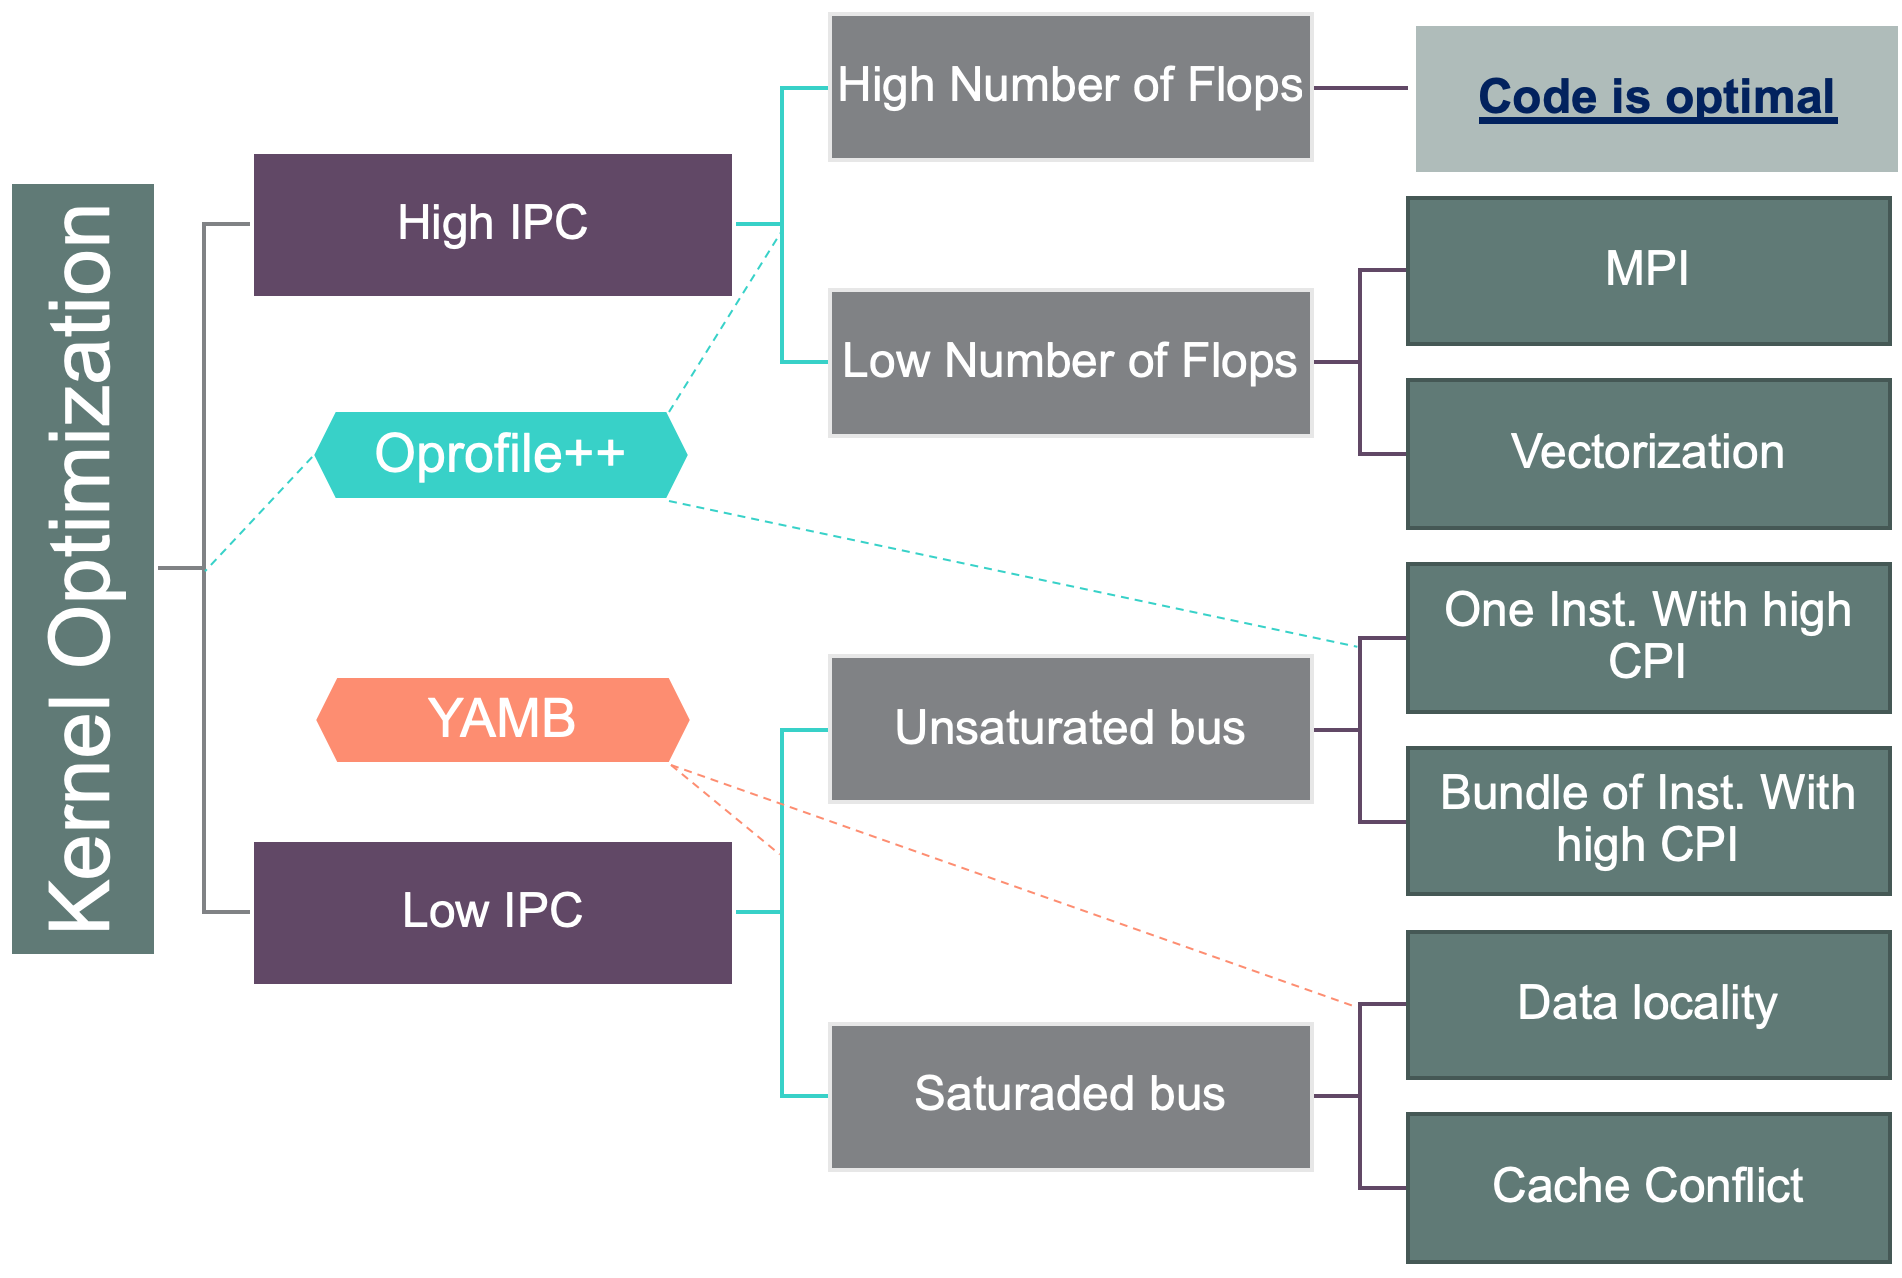
\includegraphics[width=12cm]{images/analyse_bigpicture.png}
            \caption{\label{pic:analyse_bigpicture} Flux de travail pour l'utilisation des outils \textit{Oprofile++} et \textit{YAMB}. En fonction des observations amenées par les outils, des réponses différentes sont proposées au programmeur pour optimiser son code.}
        \end{figure}

        La première mesure à réaliser est celle de l'IPC des boucles critiques du noyau. Pour ce faire, nous avons présenté l'outil \verb=Oprofile++= dans la \autoref{sec:oprofile} (voir \autoref{lst:oprofileex}). Si l'outil indique un IPC faible, il y a de fortes chances que le système mémoire soit responsable de la mauvaise performance. Un IPC élevé indique quand à lui que le problème vient du processeur.
        
        \begin{lstlisting}[language={},caption=L'outil \textit{Oprofile++} permet d'extraire le code assembleur et d'y associer le compteur de cycles,label={lst:oprofileex}, 
  frame=tb]
================================================================
Analysis from the app name (horner1_long) hot spot from the symbole name (f1(double)) which takes 50.1878% 
================================================================
CYCLES       INSTS      ADDRESS    disassembly
----------------------------------------------------------------
     5           11      401be0    vmovupd 0xd1b8(%rip),%ymm1
    39           79      401bf0    vfnmadd231pd 0xd1c7(%rip),%ymm11,%ymm1
     3           14      401bf9    vfmadd213pd %ymm2,%ymm11,%ymm1
...
   760         1652      401c3e    cmp    %eax,%edx
    48           99      401c40    jb     401be0 <_Z8range_f1ddi+0xa0>
----------------------------------------------------------------
LOOP from 401c40 to 401be0  size= 96 sum(cycles)= 2287 
     IPC= 2.12462 cycles/LOOP= 10.3548 flop/cycle = 1.42 
----------------------------------------------------------------
\end{lstlisting}

        
        \subsubsection{Profilage de la mémoire}
        %%%%%%%%%%%%%%%%%
            Lorsque la première analyse indique que la mauvaise performance du noyau est dûe au système mémoire il est nécessaire de réaliser l'analyse de son activité. La première vérification à faire et de s'assurer que le bus mémoire est saturé. Pour y répondre, nous proposons d'utiliser l'outil YAMB (voir \autoref{sec:yamb}) qui affiche l'activité du bus mémoire (lecture, écriture et utilisation totale). Pour confirmer sa saturation, il est nécessaire d'avoir caractérisé la performance du bus mémoire lors de la première étape et d'en connaître la performance maximale. 
            
            Pour valider sa saturation, il est important de posséder une fréquence d'échantillonage suffisamment élevée. En effet, avec une fréquence trop faible, il peut arriver que le graphique montre une saturation avec une ligne droite atteignant la performance maximale. En augmentant le fréquence et en grossissant certaines parties du graphique, il est possible de voir que le bus n'est pas totalement utilisé pendant des périodes très courtes, et saturé quelques cycles après. Ce phénomène peut être dû à des dépendances entres plusieurs instructions. Des techniques de déroulement de boucles sont alors très efficaces si la nature de l'application le permet (voir \autoref{sec:dml_unroll}). Un autre facteur peut venir de la mauvaise gestion du préchargement des données. Il peut alors être intéressant de réaliser le préchargement manuellement en démarrant les chargement de données plusieurs instructions avant qu'elles soient utilisées. D'autres techniques, telles que la fusion de différentes boucles (ou noyau) nous ont permis d'améliorer la performance de plusieurs applications.
            
            Si le bus est bien saturé, nous utilisons le modèle SMM pour comparer les ratio de lecture/écriture avec celui calculé dans l'étape 1 (voir \autoref{sec:smm}). Un mauvais ratio peut provenir d'un nombre de lectures plus élevé que prévu. En effet, il est très rare de réaliser plus d'écriture que nécessaire. Ceci est causé par un large éventail de problèmes potentiels, par exemple, des conflits dans le cache, la lecture de données inutiles, une décomposition incorrecte des données ou des structures de mémoire inappropriées. Pour y remédier, des techniques de \textit{blocking} peuvent être utilisées pour améliorer l'utilisation de la localité des données.  L'outil aide pour trouver si des groupes d'instructions sont plus long à exécuter que d'autres, pouvant être expliqué par une dépendance entre les données ou une donnée non présente dans la mémoire cache au moment requis. 
        
        
        
        \subsubsection{Profilage du processeur}
        %%%%%%%%%%%%%%%%%
        
            Si la première analyse montrait que la mauvaise performance n'était pas dû au système mémoire, il faut alors affiner l'analyse de l'exécution du code donnée par \verb=Oprofile++= (voir \autoref{lst:oprofileex}).
            La première vérification à faire est de compter le nombre d'opérations flottantes réalisées par la boucle. Pour cela, nous comptons manuellement le nombre d'opérations flottantes à partir des instructions assembleurs utilisées. Si le nombre d'opérations flottantes et l'IPC sont élevés, cela indique que le code est optimal. 
            
            Un nombre d'opérations flottantes faible associé à un IPC élevé indiquent que la parallélisation n'est pas correctement utilisée. Il est alors conseillé de regarder le type d'instructions exécutées.
                Un compilateur de mauvaise qualité aura tendance à générer de nombreuses instructions supplémentaires simple à exécuter. Cela fait augmenter l'IPC de la boucle sans en améliorer la performance. Un mauvais compilateur aura tendance à générer plus d'instructions qu'un bon compilateur pour le calcul d'adressage par exemple. La performance du code peut alors être limitée par l'unité de calcul d'adresses et non par la FPU.
                Un autre exemple couramment rencontré est l'exécution d'instructions de la librairie MPI utilisée pour synchroniser les processus. Celles-ci sont exécutées à chaque cycle pour vérifier l'état des autres processus, faisant augmenter l'IPC de la boucle. Il faut alors utiliser des outils tels que Paraver, Extrae ou Vampire pour vérifier que la répartition du travail est bien réalisée. Un noeud de calcul ayant un matériel défectueux affectent alors les autres serveurs, et de nombreux cycles sont perdus dans ces instructions de synchronisation. Les pannes sont très difficiles à identifier sans les outils adaptés car ils peuvent venir d'une mutlitude d'endroits: barette mémoire défectueuse, surchauffe du processeur ou un disque cassé.
                Si la boucle contient beaucoup d'instructions de calculs flottantes, il faut vérifier qu'il s'agit d'instructions vectorielles les plus larges possibles.
            
            Il est donc important de ne pas baser son analyse que sur la lecture de l'IPC mais de vérifier que les instructions exécutées sont des instructions de calculs flottants. Les transformations du code nécessaires pour y parvenir peuvent être difficile à réaliser et demander l'utilisation d'un autre algorithmes ou de restructurer le jeu de données.
            


%%%%%%%%%%%%%%%%%
\subsection{Application au benchmark \textit{Stream}}
%%%%%%%%%%%%%%%%%

    Nous appliquons notre méthodologie sur le benchmark Stream fonctionnant sur un processeur Intel Skylake. Cet exercice nous permet de montrer que même sur un code aussi simple, apparemment optimal, notre analyse nous permet de comprendre sa performance et de l'optimiser.
    
        
    \subsubsection{Vérification du modèle SMM}
    %%%%%%%%%%%%%%%%%
    
        Nous avons montré précédemment que la performance du noyau était limitée par la bande passante mémoire. Nous avons appliqué notre modèle de performance SMM et déterminé $\text{TEMPS}_{optimal}$ égale à $\frac{58.8}{128} = 0.56$ seconde. En utilisant la fonction présenté dans l'\autoref{lst:gettime} nous mesurons $\text{TEMPS}_{mesure} = 0.79$ seconde.
        L'application n'est donc pas optimale. Ceci est également validé par le résultat du benchmark Stream qui annonce une bande passante mémoire de 80,13 GB/sec (à l'aide de \verb=DML_MEM= nous avions mesuré $\text{MEMORY}_{max} = 105 GB/s$).
        
        Pour comprendre ce résultat, nous avons utilisé YAMB pour vérifier que le bus mémoire était bien saturé. Le graphique de la \autoref{fig:stream_before} nous montre que le bus mémoire est utilisé au maximum de son potentiel de 104 GB/s. La saturation du bus n'est donc pas la cause de la mauvaise performance du noyau. Il est alors nécessaire de regarder les rapports lecture/écriture. Lors de l'étape 3, nous avions calculé un ratio optimale pour ce noyau  d'une écriture pour deux lectures. La \autoref{fig:stream_before} montre la répartition mesurée lors de l'exécution: 26 GB/s en écriture pour 78 GB/s en lecture, pour un total de 104 GB/s, ce qui correspond à un ratio de 1 écriture pour 3 lectures. Ce ratio exact d'une écriture pour trois lectures n'est pas une coïncidence. Un vecteur entier est lu alors qu'il ne devrait pas l'être.
        
        \begin{figure}[htb]
        {
        \centering
        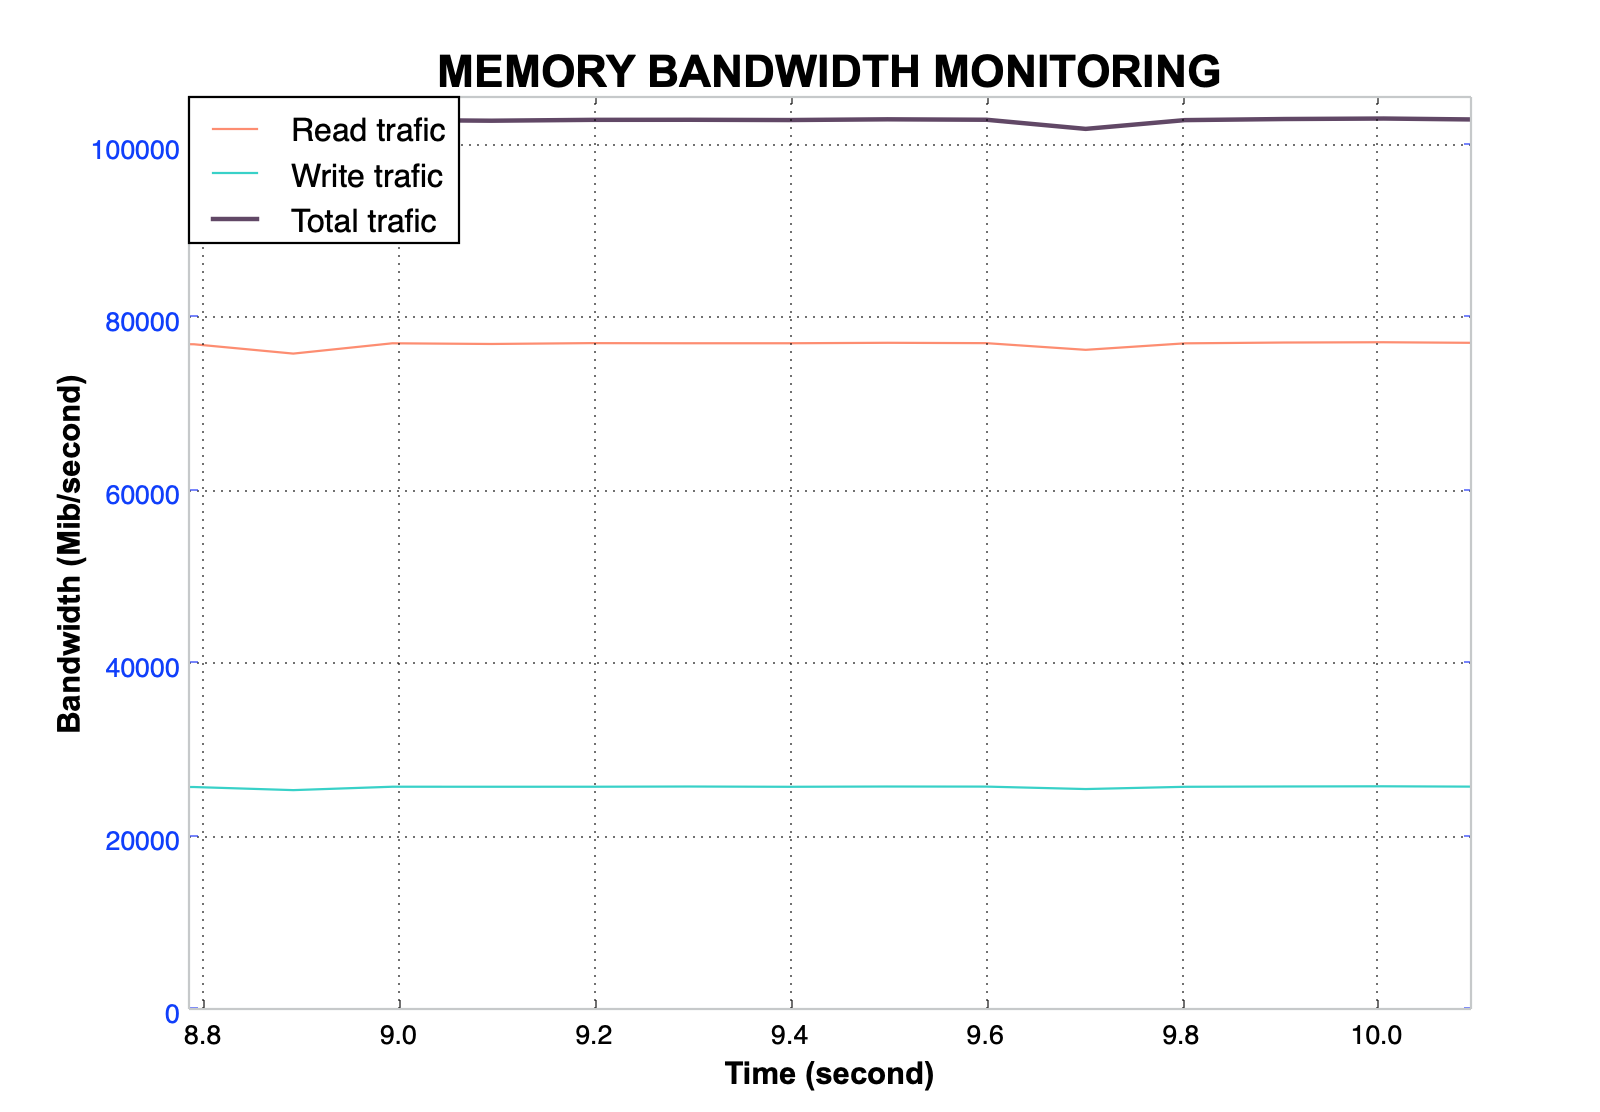
\includegraphics[width=0.80\textwidth]{images/stream_before.png}
        \caption{Prolie mémoire donné par l'outil YAMB pour plusieurs exécution de noyau \textit{triadd} du benchmark \textit{Stream}. }\label{fig:stream_before}
        }
        \end{figure}


        
        \subsubsection{Optimisation du noyau \textit{triadd}}
        %%%%%%%%%%%%%%%%%
            
            Les deux vecteurs B et C doivent nécessairement être lus une fois. La lecture supplémentaire provient du vecteur en écriture. Ce comportement est dû au processeur qui, avant d'écrire une donnée, charge la ligne de cache correspondante pour la mettre à jour. Cependant, le noyau étudié a la particularité d'écrire toute la ligne de cache, les données initialement présentes n'ayant aucune valeur utile. Une option peut être utilisée avec le compilateur Intel (ICC) pour permettre au compilateur d'éviter ce chargement inutile: \verb|-qopt- streaming-stores=always|. Cette option permet au CPU d'écrire toute la ligne de cache sans avoir à la charger.
            
        
        \subsubsection{Performance du noyau optimisé}
        %%%%%%%%%%%%%%%%%
        
            Nous avons compilé \textit{Stream} avec l'option \textit{-qopt- streaming-stores=always} et mesuré le temps et la bande passante de la même manière que pour la première exécution. Les résultats sont résumés dans le \autoref{table:stream_res}. Le temps passé dans le noyau est de 0,59 seconde, beaucoup plus proche du maximum théorique de 0,56 seconde. En analysant la bande passante mémoire, on constate que le rapport lecture/écriture est maintenant de 2 pour 1, les données échangées étant de 34 GB/s en mode écriture pour 68 GB/s en mode lecture. La bande passante total atteint 104 GB/s proche $\text{MEMORY}_{max}$.
            
            %\renewcommand{\arraystretch}{1.2}
            %\setlength{\tabcolsep}{8pt}
            
            \begin{table}[htbp]
            \centering
            \caption{Performance du noyau \textit{triadd} du benchmark \textit{Stream} avant et après optimisation. Le temps (seconde) après optimisation est proche de l'optimum théorique $\text{TEMPS}_{optimal}$  calculé à 0,56 sec. L'utilisation du bus mémoire est approximativement la même entre les deux versions du code (104 et 102 GB/s). L'option de compilation optimise le rapport lecture/écriture (GB/s) et améliore les performances du code de 25\%.}
            \begin{tabular}{l|c|c|c|c|c|}
            \cline{2-6}
            & $\text{TEMPS}_{mesure} (s)$ & Stream   & $\text{YAMB}_{read}$  & $\text{YAMB}_{write}$  & $\text{YAMB}_{total}$  \\ \hline
            \multicolumn{1}{|l|}{Version originale}  & 0.79   & 80.13  & 26        & 78         & 104        \\ \hline
            \multicolumn{1}{|l|}{Version optimisée} & 0.59   & 101.84 & 35        & 69         & 104        \\ \hline
            \end{tabular}
            \label{table:stream_res}
            \end{table}
    

\subsection{Travaux liés}
\url{https://tel.archives-ouvertes.fr/tel-00984791v4/document}


\subsection{Conclusion}
%%%%%%%%%%%%%%%%%

\textbf{TODO}
\begin{itemize}
    \item Through this experiment we wanted to show that having a solid analytic methodology is essential to understand the performance of a code
    \item Only measuring the memory throughput is not enough to conclude that the code is optimal. 
\end{itemize}


\printbibliography[heading=references,segment=\therefsegment]
